\documentclass[12pt]{report}
\usepackage[utf8]{inputenc}

\title{SPATIAL ENHANCEMENT OF REMOTELY SENSED IMAGES USING CONVOLUTIONAL NEURAL NETWORKS}
\author{Palatucci Ugo}
\date{July 2020}

\usepackage{graphicx}
\usepackage{url}
\usepackage{amsmath}
\usepackage[margin=1.5in]{geometry}
\usepackage{listings}
\usepackage{setspace}
\usepackage{longtable}
\usepackage{xcolor}
\newcommand{\rr}[1]{\textcolor{red}{\textbf{#1}}}
\newcommand{\bb}[1]{\textcolor{blue}{\textbf{#1}}}

\linespread{1.75}

\begin{document}
\newgeometry{margin=1.5in}

\begin{titlepage}
    \begin{center}
        \vspace*{1cm}
            
        \large
        \textbf{SPATIAL ENHANCEMENT OF REMOTELY SENSED IMAGES USING CONVOLUTIONAL NEURAL NETWORKS}
            
        \vspace{0.5cm}
            
        Ugo Palatucci
            
        \vspace{0.25cm}

        July 2020
            
        \vspace{0.8cm}
            
        \begin{figure}[!ht]
            \centering
            
\includegraphics[scale=.5]{unisa.png}
        \end{figure}
            
    \end{center}
    Supervisor: \newline
    Prof. Restaino Rocco
    
\end{titlepage}

\restoregeometry

\tableofcontents

\chapter*{Introduction}
\addcontentsline{toc}{chapter}{Introduction}
Pansharpening refers to a particular data fusion issue where two images, one panchromatic (PAN) and one multispectral (MS), representing the same area can be combined to enhance the peculiarity of both. The panchromatic image is acquired with a wide spectrum sensor that can have a higher spatial resolution compared to a multispectral one. However, the sensor cannot acquire different bands. A multispectral sensor, instead, collects several channels at a lower spatial resolution. As physical constraints occur, the creation of a sensor specialized in both types of resolution would not be possible. For this reason, the fusion of both images can be the only possibility to have a new image with higher spatial and spectral resolution. Pansharpening is an urgent topic for remote sensing; indeed, the result can be used upstream of another process such as change detection \cite{changedetection}, object recognition \cite{objectrecognition}, visual image analysis and scene interpretation \cite{sceneinterp}.

Based on a convolutional neural network, a new pansharpening method has been proposed recently \cite{pnn}.
Using degraded versions of the PAN and MS images, the network weights were trained to fuse the images, optimizing a reference index with the gradient descendent algorithm: the mean squared error. After the training, the same weights were applied to fuse the original PAN and MS images.

The purpose of this work is to improve the current methodology using the original PAN and MS images for a training with a \textit{no-reference} index like Quality with no reference (QNR) or hybrid QNR (HQNR) indexes. Furthermore, the intention is to remove the error added using the degraded images that do not reflect the models were the pansharpening algorithm should be utilised.
In \cite{pnn} the code was written in python 2.7 using the Theano library. The Theano project has been not updated since 2018 \cite{theanorip}. For this reason, the project is incompatible with new Cuda libraries and NVIDIA drivers and many issues to run the training process on the GPU have been founded. To solve that, a new software has been created using TensorFlow. Tensorflow is a more modern and popular Deep Learning library maintained by Google that allows more compatibility with the newest libraries and a larger community, helping the development in case of uncommon errors. 
Moreover, Tensorflow implements the \emph{automatic differentiation} \cite{tensorflowautoderiv}, a critical feature for this research. \emph{Automatic differentiation} allows writing differentiable functions and subsequently using them for the core algorithm of the neural network's backpropagation training: the gradient descendent algorithm. 


\chapter{Pansharpening state of the art}


According to the existing literature, the pansharpening techniques are divided into two main areas: \textit{component substitution} (CS) and \textit{multiresolution analysis} (MRA). The techniques belonging to the first class consist in representing the MS and PAN in a different domain that can entirely split the spatial information from the spectral information. In this domain, the spatial information part of the MS image can be replaced with the PAN image. After this substitution, the MS image can be back-transformed in the original domain. Clearly, the less the PAN is correlated with the replaced component, the more distortion is introduced. The most famous techniques of this class are intensity-hue-saturation (IHS) \cite{ihs1, ihs2}, in which the images are represented in the IHS domain, principal component analysis (PCA) \cite{scaleinvariance1, pca2} and Gram-Schmidt (GS) spectral sharpening \cite{gs}. On the one side, those techniques preserve the PAN spatial information. On the other side they can produce a high spectral distortion. This is because PAN and MS are obtained in spectral ranges that only partially overlap. 

The second class of techniques, MRA, are based on the introduction of spatial details, extracted from the PAN image through a multgiscale decomposition, into the up-sampled version of the MS. This approach promises a better spectral fidelity but often present spatial distortions.

The lack of the reference image is the principal issue in the evaluation of the pansharpening methods.
When a couple of images are fused, the result cannot be compared with anything else. The sensors used for the acquisition cannot reach alone both spatial and spectral resolution of the result. As the two models are different, the result cannot be compared with another image acquired with a different sensor.
For this reason, there is no universal measure of quality for the pansharpening. The scientific community common practice is to use the verification criteria that were proposed in the most credited work \cite{towaldetal}. This study defines two properties to use for the evaluation of the fused product: consistency and synthesis. The first means that the original MS image should be obtained with a degradation of the fused result.
The second property describe that the fused image should preserve both the features of each band and the mutual relations among them. The definitions of an algorithm that accomplishes these properties and of an index that can guarantee the correct evaluation are an open problem. But, no matter what index is decided to use, the unavailability of a reference image is a huge problem and a visual inspection is always mandatory. 

Accordingly, there are two techniques that can be used for the quality assessment. The first is to degrade both the images given in input to the pansharpening algorithm and use the original MS image as a reference for the result evaluation. The downside of this method is the assumption of invariance between scales, which justifies that the same algorithm operates similarly at reduced scale. The cited hypothesis  is not always verified as documented in \cite{scaleinvariance1, towaldetal}. A second technique is the use of an index that does not require a reference image.


\section{CS}

The CS family is based on converting the MS image into a domain in which the spatial and spectral pieces of information can be better separated. In this domain, the component containing the spatial information can be replaced by the PAN image. The greater the correlation between the PAN image and the replaced component, the lower the distortion introduced by the fusion. For this reason, the histogram matching of the PAN with the component that contains the spatial part of the MS information is preliminarily performed.
After the substitution, the data can be represented in the original space with an inverse transformation. This approach is applied to the whole image in the same way. Techniques of this category have high fidelity regarding the fusion of spatial details and are fast and easy to implement. But as the acquisition spectrum of the sensors used to produce the PAN and MS image differ each other, the process may produce significant spectral distortions \cite{cs1,cs2}. 
In the studies \cite{cs3,cs4,cs5,cs6,cs7}, it was shown that, when a linear transformation is used, the substitution and fusion can be obtained without the explicit forward and backward transformation of the images but with a precise injection scheme. This scheme can be formalized according to the following equation:
 %
\begin{equation}
    \widehat{MS_k} = \widetilde{MS_k} + g_k(P - I_L), \qquad k = 1,\dots,N
    \label{cs}
\end{equation}
%
in which $k$ indexes the spectral bands, $g_k$ are the injection gains, $\widehat{MS_k}$ is the $k$-th band of the pansharpened image, $\widetilde{MS}_k$ is the $k$-th band of the MS image interpolated to the PAN scale and $I_L$ is the intensity component derived from the MS image according to the relation:
% 
\begin{equation}
    I_L = \sum_{i=1}^{N} w_i\widetilde{MS_i}
    \label{ilcs}
\end{equation}
%
The weight vector $w= [w_1,w_2, \ldots,w_k] $ is the first row of the forward transformation matrix and depends on the spectral overlap among MS channels and PAN.
 

\begin{figure}[t!]
\centering
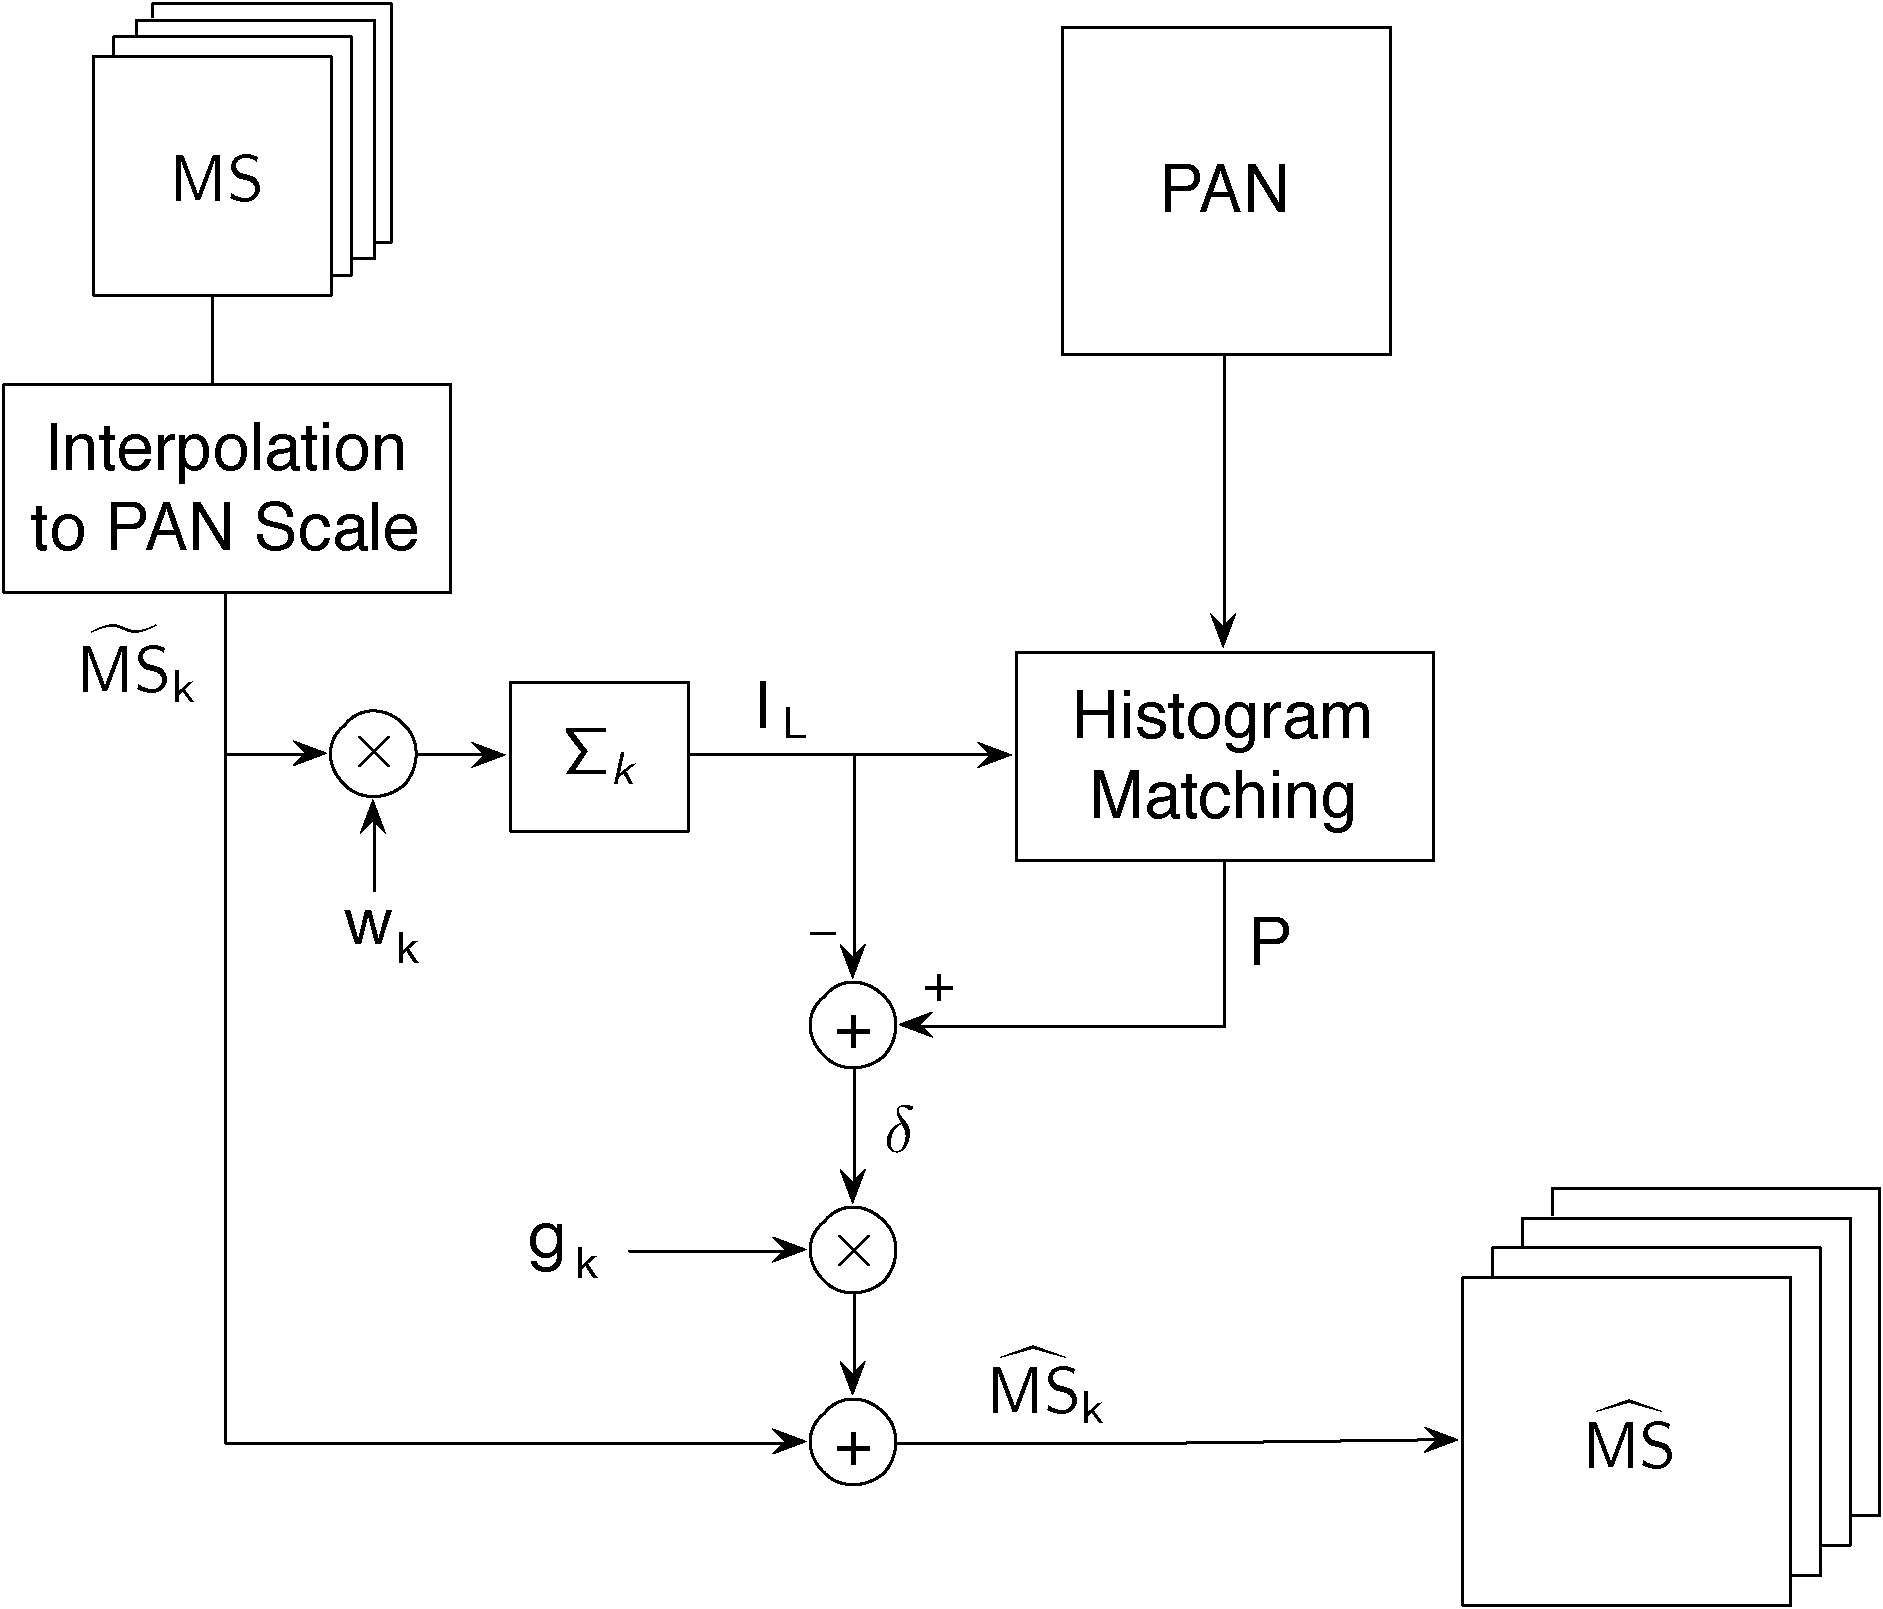
\includegraphics[width=0.9\textwidth]{cs.png}
\caption{Flowchart of CS approach \cite{criticalComparison}.}
\label{fig:csapproach}
\end{figure}


The CS approach procedure is illustrated in  Fig.~\ref{fig:csapproach}. Four important steps can be noticed: 
1) interpolation of MS image for matching the PAN scale; 2) calculation of $I_L$ using Eq.~(\ref{ilcs}); 3) histogram matching between PAN and intensity component; 4) details injection according to Eq.~(\ref{cs}).

The various CS techniques such as IHS \cite{ihs1,ihs2}, PCA \cite{pca2,changedetection} and GS \cite{gs,cs3} define different $w_{k,i}$ and $g_k$.

In the IHS pansharpening method the IHS transformation is used. This is the major limitation of this technique because it can transform only RGB images and often the MS image has 4 or also 8 and more bands. As a workaround, the authors of paper \cite{cs6} has proved that GIHS, a generalization of the IHS transformation for more bands, can be formulated for any arbitrary set of nonnegative spectral weights as described in the following equation: 
%
\begin{equation}
    \widehat{MS_k} = \widetilde{MS_k} + \left(\sum_{i=1}^{N}w_i\right)^{-1}(P - I_L), \qquad 
    k = 1,\dots,N
    \label{cs2}
\end{equation}
%
in which $w_i$ are all equal to $1/N$ \cite{ihs1}.

With the injection gains defined such that:
\begin{equation}
    g_k = \frac{\widetilde{MS_k}}{I_L}, \qquad k = 1,\dots,N
    \label{csgk}
\end{equation}
%
$\widehat{MS_k}$ can be calculated as 
\begin{equation}
    \widehat{MS_k} = \widetilde{MS_k} \cdot \frac{P}{I_L}
    \label{csfinal}
\end{equation}
%
which is the well-known Brovey Transform. 

In the PCA pansharpening method, it is used the PCA transformation, also called Karhunen-Loeve transform. It is a linear transformation that can be implemented for a multidimensional image, so it is not limited as the IHS method, and consists into the projection of all the components along the eigenvectors of the covariance matrix. This means that each component is orthogonal and statistically uncorrelated from the others. The hypothesis introduced in this step is that the spatial information is concentrated in the first component, the component with the larger eigenvalue. The PCA can be implemented by using Eq.~(\ref{cs}), in which $w$ is the first row of the forward transformation matrix; $g$ is the first column of the backward transformation matrix.

The GS transformation is a common technique used to orthogonalize a set of vectors in linear algebra.
First of all, the $\widetilde{MS}$ bands are organized in vectors to obtain a two dimensional matrix in which the columns are constituted by the bands organized as vectors. The mean of each band is subtracted from all the columns. The orthogonalization procedure is used to create a low-resolution version of the PAN image, i.e., $I_L$.  The last step is the replacement of $I_L$ with the histogram matched PAN before the inverse transformation. GS is a generalization of PCA in which PC1 may be any component and the remaining ones are calculated to be orthogonal with PC1. Also the GS procedure can be described by Eq.~(\ref{cs}) if $g_k$ is defined as:
%
\begin{equation}
    g_k = \frac{\operatorname{cov}(\widetilde{MS_k}, I_L)}{\operatorname{var}(I_L)} , \qquad k = 1,\dots,N
    \label{gsgk}
\end{equation}
%
in which $\operatorname{cov}(\cdot,\cdot)$ is the covariance between two images and $\operatorname{var}(\cdot)$ is the variance.
There are several versions of this technique that differ on how the $I_L$ is
created. The simplest way is to set $w_i = 1/N$. This version is called 
GS mode 1~\cite{gs}. In~\cite{cs3}, also an $adaptive$ version of this mode was proposed. It is called GSA and the $I_L$ is generated by a weighted average of 
the MS bands. Another technique defined in \cite{gs} and called GS mode 2 
suggests to generate the $I_L$ by applying a low pass filter to the PAN image. 
This last step leads the GS mode 2 that belongs to the MRA class of techniques.

Another noteworthy technique is described in \cite{cs7} and introduces the concept of 
\textit{partial replacement} of the intensity component. An intensity
image is created  for every band of the MS from the PAN image; it is calculated with the following equation:
%
\begin{equation}
    P^{(k)} = CC(I_L, \widetilde{MS_k}) \cdot P + (1 - CC(I_L, \widetilde{MS_k})) \cdot 
    \widetilde{MS_k^{'}}
    \label{pk}
\end{equation}
%
in which $\widetilde{MS_k^{'}}$ is the $k$-th MS band histogram-matched to PAN and CC is the
correlation coefficient.
$I_L$ is defined using in Eq.~(\ref{ilcs}) a vector $w$  obtained with a linear regression of $\widetilde{MS_k^{'}}$
on $P_L$, the degraded version of the PAN.
The injection gains are the result of:
%
\begin{equation}
    g_k = \beta \cdot CC(P_L^{(k)}, \widetilde{MS_k}) \cdot 
    \frac{std(\widetilde{MS_k})}{\frac{1}{N}\sum_{i=1}^N std(\widetilde{MS_i}))} L_k
    \label{gkpk}
\end{equation}
%
$\beta$ is empirically tuned and is a factor that normalizes the high frequencies.
$P_L^{(k)}$ is a low-pass-filtered version of  $P^{(k)}$,  and $L_k$ is an adaptive factor 
that removes the local spectral instability error between the synthetic component image 
and the MS band defined as:
%
\begin{equation}
    L_k = 1 - \left|1 - CC(I_L, \widetilde{MS_k})\frac{\widetilde{MS_k}}{P_L^{(k)}}\right|.
    \label{lk}
\end{equation}
%

\section{MRA}

In the MRA class of techniques, the pansharpened image is defined as:
%
\begin{equation}
    \widehat{MS_k} = \widetilde{MS_k} + g_k(P - P_L), \qquad k = 1,\dots,N. 
    \label{mra}
\end{equation}
%
$P - P_L$  is the operation performed to obtain the high-frequency details of the PAN image. 
The algorithm to create the $P_L$ and the chosen $g_k$ weights differentiate the MRA 
pansharpening techniques of this class.

\begin{figure}[t!]
\centering
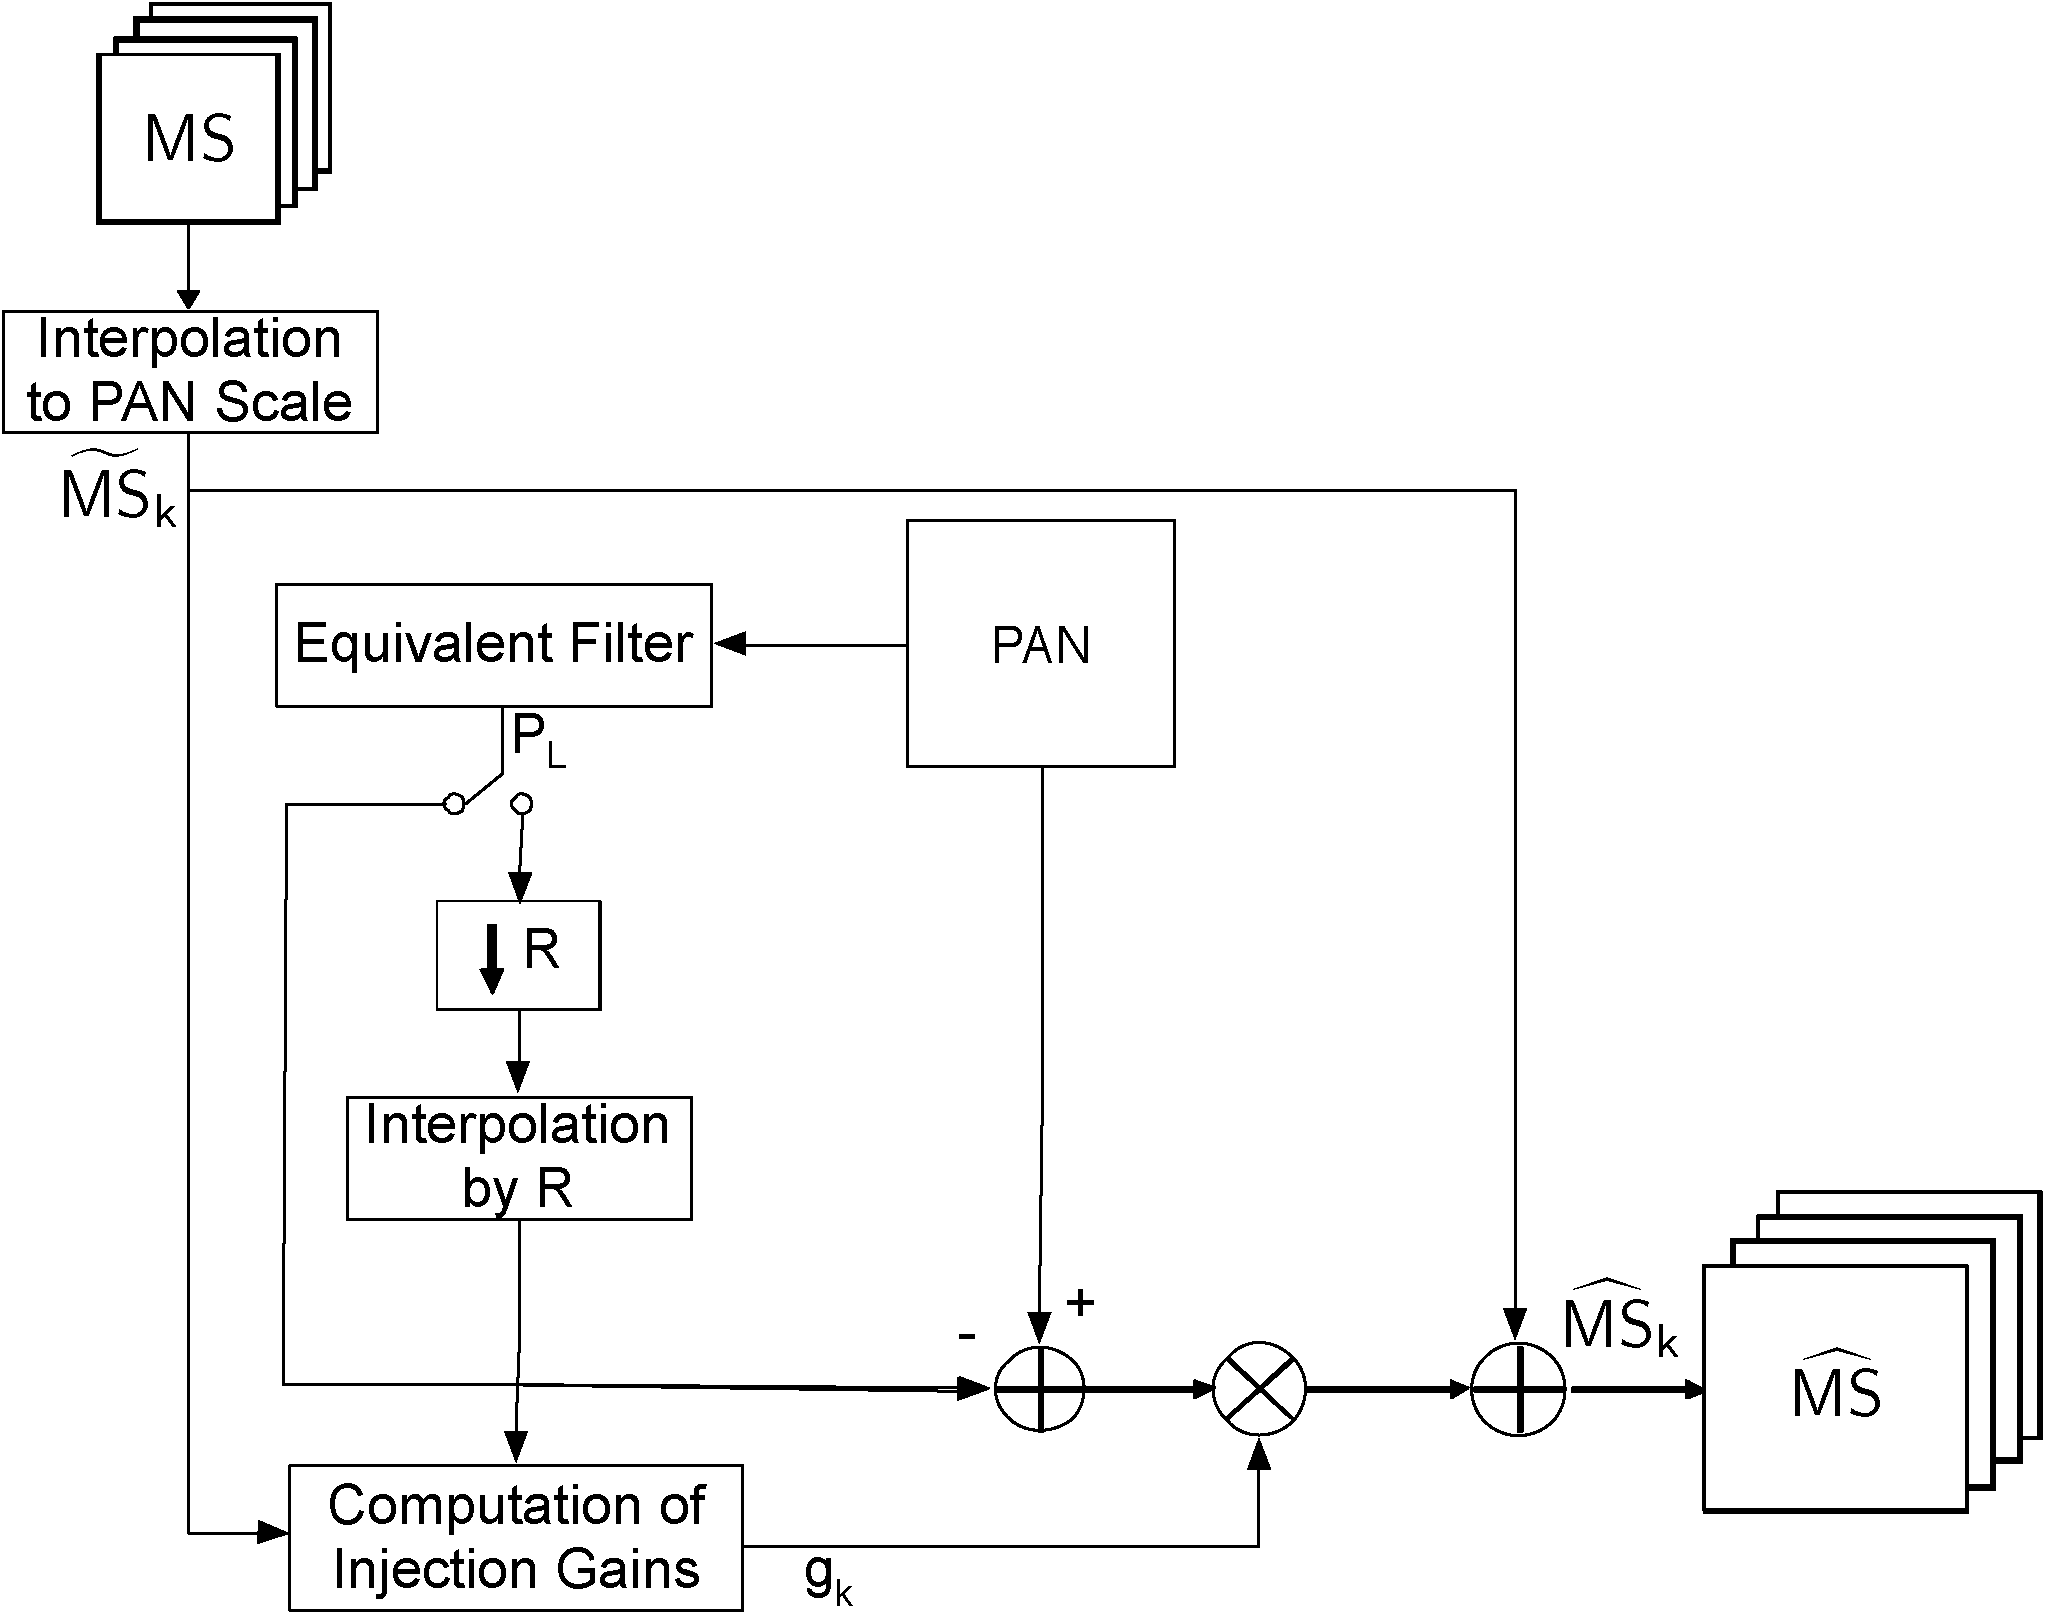
\includegraphics[width=0.9\textwidth]{mra.png}
\caption{Flowchart of MRA approach \cite{criticalComparison}}
\label{fig:mraapproach}
\end{figure}

However, in general, all the techniques follow the algorithm described in Fig.~\ref{fig:mraapproach}. 
First of all, the MS image is interpolated to the PAN scale.
The second step is to calculate $P_L$, the low pass version of PAN obtained by means of an equivalent filter.
The vector of injection weights $g_k$ can be computed using the $\widetilde{MS_k}$ in combination with $P_L$.
Interpolation is less crucial in MRA respect to CS methods.
A method to produce the $P_L$ image consists in applying a low pass filter $h_{LP}$ to the PAN image $P$.
So Eq.~(\ref{fig:mraapproach}) can be rewritten as:
%
\begin{equation}
    \widehat{MS_k} = \widetilde{MS_k} + g_k(P-P*h_{LP}), \qquad k=1,\dots,N
    \label{mra1}
\end{equation}
%
where $*$ is the convolution operation.
A more general method to obtain the $P_L$ is called \textit{Pyramidal Decompositions} and the number of 
filterings can be one or more. A filter type that proves to be a good choice is a Gaussian filter that closely 
matches the sensor MTF. A noteworthy option is the MTF-GLP with a context-based decision (MTF-GLP-CBD) \cite{mtfglp}
where the injection gains are defined as follows: 
%
\begin{equation}
    g_k = \frac{cov(\widetilde{MS_k}, P_L^{(k)})}{var(P_L^{(k)})}
    \label{mragk}
\end{equation}
 It is context-based because it can be applied on nonoverlapping image patches to improve the quality of the final product.

\section{Quality Assessment}
As explained above, the lack of a reference image is the main limitation. The community has proposed two assessment
procedures as a workaround. The first procedure consists in using the images at a lower spatial 
resolution and keeping the original MS image as a reference. However, the output of an algorithm can have 
different performance at different scales, as it is showed in~\cite{perfdiffscale}.
This happens because the performance assessment depends intrinsically on the image scale, 
mostly in case of pansharpening methods that apply spatial filters.
The second procedure consists in using non-reference quality indexes. 
Both types of procedures require also a visual inspection for spectral distortions and spatial details.

The Wald's protocol is composed by three requirements:
\begin{enumerate}
	\item $\widehat{MS_k}$ degraded to the original MS scale should be as identical as possible to the $MS_k$.
    \item The fused image $\widehat{MS_k}$ should be as identical as possible to the $MS_k$ that the sensor would acquire at the highest resolution
    \item The MS set of synthetic images $\widehat{MS} = {\{\widehat{MS}\}_{k=1,\dots,N}}$ should be as identical as possible
    to the MS set of images $HRMS = \{HRMS\}_{k=1,\dots,N}$ that the corresponding sensor would observe at the highest resolution.
\end{enumerate}

In the previous definitions, HRMS is the reference image.
For a reduced-resolution assessment, the filter choice for the downsampling is crucial in the validation. 
A bad filter choice results in an image degradation that does not reflect the 
sensor characteristics at a lower scale. So the algorithm, after the degradation, is applied to
images that reflect the wrong sensor model. This means that the same algorithm can have a more different result at the original and lower scales. On the contrary, with a good filter that preserves the sensor characteristics at the lower resolution, the algorithm has a higher  possibility to reflect the quality of the original resolution.
Indeed, the filter used for the MS degradation should simulate the transfer function of the remote sensor and so, it should match the sensor's MTF~\cite{mtfsensor}. 
Similarly, the PAN image has to be degraded in order to contain the details that would have been seen if the image were acquired at the reduced resolution.
The fused image obtained from the degraded PAN and MS, can be evaluated by means of different indexes using the MS as a reference image.

The \textit{Spectral Angle Mapper }(SAM) is a vector measure that is useful to evaluate the spectral distortion.
In simple terms, denoting by $I_{(n)} = [I_{1,{n}}, \dots , I_{N,{n}}]$ a pixel vector of the MS image, with $N$ bands,
the SAM between the corresponding pixel vectors of two images is defined as:
%
\begin{equation}
    SAM(I_i, J_i) = arcos\left(\frac{<I_i, J_i>}{||I_i|| || J_i||}\right)
    \label{sam}
\end{equation}
%
$<I_i, J_i>$ is the scalar product and $||I_i||$ is the vector $l_2$-norm. 
Applying this equation to every pixel results in a so-called SAM map.
Averaging all the pixel of the SAM map returns the SAM index for the whole image.
The optimal value of the SAM index is 0.

The \textit{Root Mean Square Error} (RMSE) is used to calculate the spatial/radiometric distortions.
It is defined as:
%
\begin{equation}
    RMSE(I,J) = \sqrt{E[(I-J)^2]}
    \label{rmse}
\end{equation}
%
where $E[\cdot]$ is the arithmetic mean.
The ideal value of RMSE is zero and is achieved if and only if $I = J$.
But it is not an efficient index because it is not considered the error for each band, but is global.
So, to better measure the error for each band, the \textit{Erreur Relative Globale
Adimensionnelle de Synthèse} (ERGAS) is used. 
The ERGAS index evaluates the RMSE error with a different weight for each band.
%
\begin{equation}
    ERGAS = \frac{100}{R} \sqrt{\frac{1}{N} \sum_{k=1}^N\left(\frac{RMSE(I_k, J_k)}{\mu(I_k)}\right)^2}
    \label{ergas}
\end{equation}
%
Obviously, the ERGAS is composed of a sum of RMSEs, so the optimal value is also 0.

Another important index is the \textit{Universal Image Quality Index} (UIQI) or also called Q-index, proposed in \cite{uiqi}.
Its expression is:
%
\begin{equation}
    Q(I,J) = \frac{\sigma_IJ}{\sigma_I \sigma_J} \frac{2 \bar{I}\bar{J}}{\bar{I}^2 + \bar{J}^2} 
    \frac{2 \sigma_I \sigma_J}{(\sigma_I^2 + \sigma_J^2)}
    \label{q}
\end{equation}
%
where $\sigma_{IJ}$ is the covariance of $I$ and $J$, and $\bar{I}$ is the mean of $I$.
The first fraction represents an estimation of the covariance, the second is a difference in the mean luminance
and the third is the difference in the mean contrast.
The Q-index varies in the range $[-1, 1]$ with 1 as the optimal value.


Q4 is an extension of the UIQI for images with 4 bands \cite{q4}. 
Let $a$, $b$, $c$ and $d$ denote the radiance values of the given image pixel in four bands, and construct the quaternions:
%
\begin{equation}
    z_A = a_A + ib_A + jc_A + kd_A
    \label{za}
\end{equation}
%
\begin{equation}
    z_B = a_B + ib_B + jc_B + kd_B
    \label{zb}
\end{equation}
%
The Q4 is defined as :
%
\begin{equation}
    Q4 = \frac{4 | \sigma_{z_A z_B}| \cdot |\bar{z_A}| \cdot |\bar{z_B}|}{(\sigma_{z_A}^2 + \sigma_{z_B}^2 (|z_A|^2 + |z_B|^2))}
    \label{q4}
\end{equation}
%
where $\bar{z}$ is the complex conjugate.
If eventually, the bands are more than 4, the Q4 can be replaced with Q average.

An index used for the validation at full-resolution is the \textit{Quality with no reference} (QNR) index \cite{qnr}.
It is defined by the following equation:
%
\begin{equation}
    QNR = (1-D_{\lambda})^\alpha (1 - D_S)^\beta
    \label{qnr}
\end{equation}
%
wherein $\alpha$ and $\beta$ are two coefficients which can be tuned to weight more
the spectral or the spatial distortion, respectively.

The maximum theoretical value of the index is 1 and is reached when $D_\lambda$ and $D_S$ are 0.
The spectral distortion is calculated with $D_\lambda$ using this equation:
%
\begin{equation}
    D_\lambda = \sqrt[p]{\frac{1}{N(N-1)} \sum_{i=1}^N \sum_{j=1, j \neq i}^N |d_{i,j}(MS, \widehat{MS}|^p)}
    \label{dl}
\end{equation}
%
where $d_{i,j}(MS, \widehat{MS}) = Q(MS_i, MS_j) - Q(\widehat{MS_i}, \widehat{MS_j})$, $\widehat{MS}$ is
the fused image and $p$ is a parameter typically set to one \cite{qnr}.
The objective is to create an image with the same spectral features of the original MS image.

The spatial distortion is calculated by:
%
\begin{equation}
    D_S = \sqrt[q]{\frac{1}{N} \sum_{i=1}^N |Q(\widehat{MS_i}, P) - Q(MS_i, P_{LP})|^q}
    \label{ds}
\end{equation}
%
where $P_{LP}$ is the low-resolution PAN image at the same scale of the MS image and $q$ is usually set to one \cite{qnr}.

Khan protocol \cite{khan} extends the consistency property of Wald's protocol.
The pansharpened image is considered as a sum of a lowpass term plus a high pass term.
The lowpass term is the original interpolated low resolution MS image and
the highpass term corresponds to the spatial details extracted from the PAN and injected into the MS image.
A Gaussian model of the sensor's MTF is used to build the filters. The similarity between the lowpass component and
the original MS image can be calculated using the Q4 index or any other similarity measure for images with more bands.
The similarity between PAN and the spatial component is measured as the average of UIQIs calculated using the PAN and each band of MS.
The same similarity is calculated also between the original MS and the degraded version of the PAN.

The QNR and the spectral distortion of Khan's protocol can be combined to yield another quality index, the \textit{Hybrid QNR} (HQNR) \cite{hqnr}, defined as
%
\begin{equation}
    HQNR = (1 - D_\lambda^{(K)})^\alpha (1 - D_s)^\beta
    \label{hqnr}
\end{equation}
%
in which $\alpha$ and $\beta$ are coefficients tuned to weight more the spectral or the spatial distortion, as in Eq.~(\ref{qnr}) and $D_\lambda^{(K)}$ is given by
%
\begin{equation}
    D_\lambda^{(K)} = 1 - Q4(\widehat{M}_L, M)
    \label{dlhqnr}
\end{equation}
%
$\widehat{M}_L$ indicates the fused image degraded to the resolution of the original MS image. 

%\newpage

\chapter{Pansharpening applications of Deep Learning}

%\section{Introduction}

Early works in the field of \textit{Deep Learning }(DL) have been made in the 1940s starting from the concept of \textit{Perceptron} \cite{perceptron} and afterwards in the 60s with the invention
of backpropagation, the most commonly used algorithm in the present day to train a \textit{Neural Network}.
The Neural Network is a model constituted by several neurons, that are eventually organized into different layers and have the ability to learn, extract and distinguish different features from the data given into input.
In order to obtain these capabilities, the network should be subjected to a training phase that requires a huge amount of
computational power.
As in the early 60s the computers were no powerful enough and there was not a great data availability,
DL had no reason to be implemented as today.

This approach is characterized by different phases.
One of them, the training, is a critical phase in which the model learns from new data and can differ for the type of issues that the model should solve.
In most of the cases, the model gives a prediction and the result is compared with a target. Initially, the error is calculated between the
output of the prediction and the target. After that, when the error is propagated in all the neurons of the model,
the weights of all the neurons are modified so that the next prediction for the same input will be much similar to the
target output. 
How this error is calculated and what means "similar" is established by the loss function that calculates the error.
The propagation uses a method called \textit{Gradient Descent} algorithm, that allows the network 
to understand how to change the weights and minimize the loss.
In order to use the gradient descent, the loss function must be differentiable so that
the gradient operator can be applied more times.
Many layers the net have, many times the algorithm apply the gradient to the error.

LeCun (1989) for the first time used a backpropagation algorithm to train a neural network to classify handwritten digits.

Nowadays, the data collected through internet, the incredible amount of computational power exhibited
by data centers and GPUs, the performance of this type of algorithm and a large number of applicative fields,
have encouraged the growth of Machine Learning (ML) and in particular, DL. 


\section{Neural Networks}

\subsection{Perceptron}

\begin{figure}[t]
    \centering
    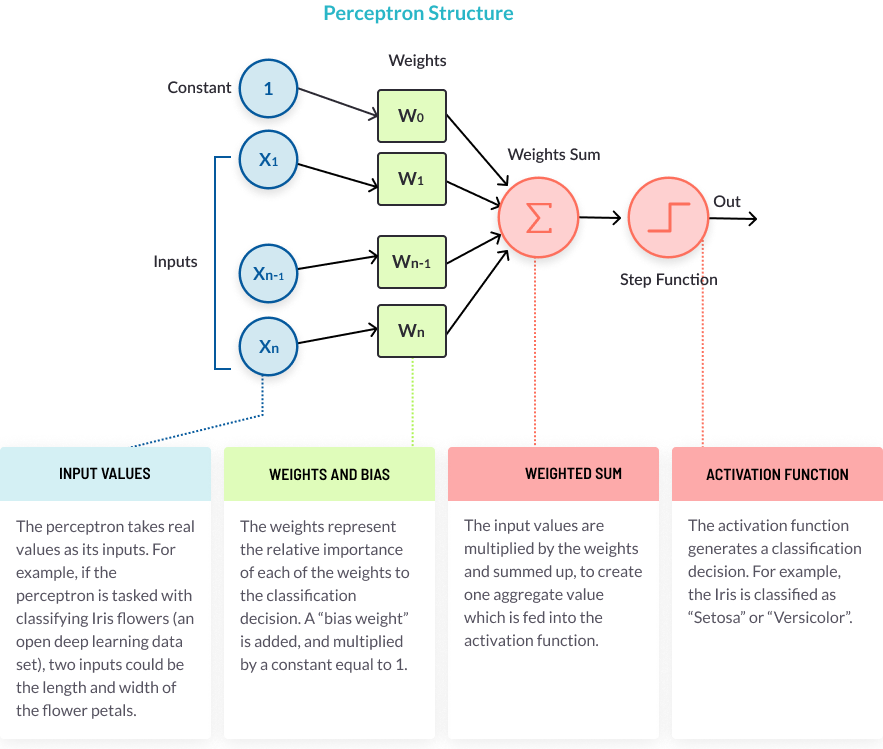
\includegraphics[width=\textwidth]{perceptron-structure.png}
    \caption{Perceptron in detail \cite{percepimage}}
    \label{fig:perceptron}
\end{figure}

Essentially a perceptron is an element in which the output is a result of a weighted sum
of the inputs. There is always only one output but it can be more inputs as depicted in Fig.~\ref{fig:perceptron}. 
A perceptron uses only one linear or non-linear activation function. The following paragraph will discuss what is an activation function and how it works.
With a non-linear transfer function, perceptron can build a nonlinear plane separating data points of different classes.
In 1969, it was proved that the perceptron itself may fail in certain simple tasks, as, for instance,
the separation of a plane described by the XOR function  \cite{xorproblem}. 
However, 3 perceptron organized in 2 layers can separate an XOR plane.
This opened up the development of multi-layer models and subsequently, for training optimization for specific
applications, the creation of different types of layers.


\subsection{Activation Function}

The activation function is used to transform the weighted data (input multiplied by weights) 
in outputs.
By the use of a non-linear transformation, we create new relation between the points.
This consents to the ML model to create increasingly complex features with every layer.
Features of many layers that use pure linear transformations can be reproduced by a single 
layer that uses a non-linear function. 
The most common activation function is the so called ReLu that
implements the relation $y = max(0, x)$, where $x$ is the input and $y$ the output. The gradient is $1$ when the value of $x$ is positive, 
and 0 when negative. This means that during the training, negative gradients will not update the weights.
A gradient equal to 1 means that the training will be much faster compared with other activation functions
like logistic sigmoid.

\subsection{Layers}

\begin{figure}[t]
    \centering
    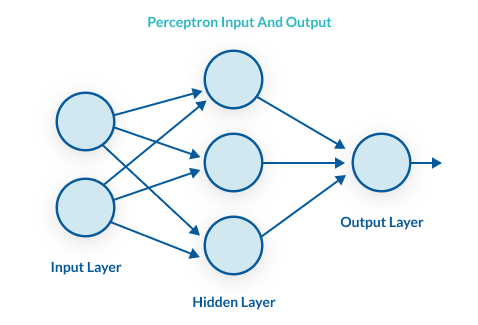
\includegraphics[scale=.5]{multilayer-perceptron.png}
    \caption{Multilayer architecture example \cite{percepimage}}
    \label{fig:multilayer}
\end{figure}

The DL network can have different type of layers that differ in how the perceptrons are organized and 
how they modify their weights during the training. 
Fig.~\ref{fig:multilayer} shows an example of a multilayer model.
The first experimented layer was the dense layer where all neurons are connected
with all neurons of the next layer. Every neuron has his own weights
and considering all the neurons connections, this type of layer generates promptly a large number of weights.
This requires a large
dataset and a long time for the training. 

The convolutional layer gave an important improvement in computer vision applications. This layer can apply different filters to the data at the same time.

Commonly, several convolutional layers at the start of a neural network are used to extract features from an image. 
In a first phase, the DL model is able to extract features in the data with complexity that grows with the model dimension, as the Fig.~\ref{fig:featuresextract} shows.
In a second phase, the features can be analyzed by different layers, for instance dense layers can elaborate features for classification or for other tasks.
The filter weights of the convolutional layer are learned in the training and applied to the whole input where the neurons share the same weights. 
For this reason, respect to a dense layer, the convolutional layer has a lower weights count, is much faster to train and allocates a minor amount of memory.

To recognize patterns among a sequence of data such as video or audio, \textit{Long short-term memory} (LSTM) \cite{lstm}  and \textit{Gated Recurrent Unit} (GRU) \cite{gru} are used
and, unlike standard layers, have feedback connections that allow the model to memorize data for subsequent inputs.
Other layers like the pooling layer, max-pooling layer and dropout were created to optimize the training.


\begin{figure}[t]
    \centering
    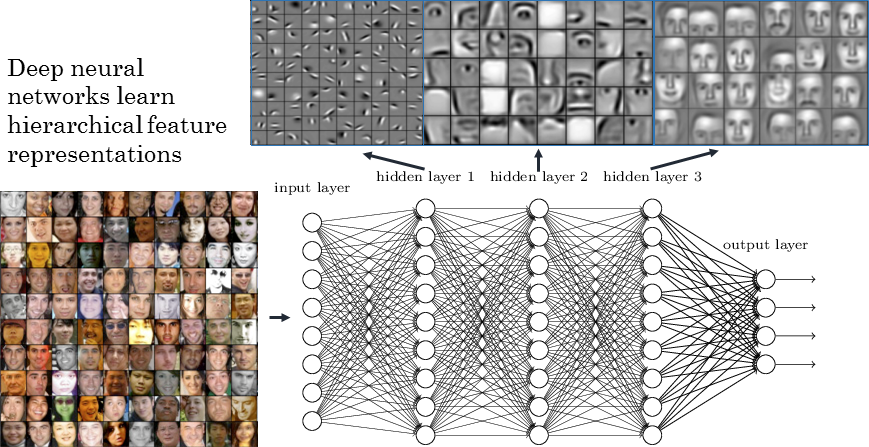
\includegraphics[scale=.5]{layers-features.png}
    \caption{Feature extraction of a deep model \cite{featuresextract}}
    \label{fig:featuresextract}
\end{figure}


\section{The Deep Learning Paradigm}

Deep Learning \cite{deeplearning} is a subfield of ML focalized in the study of deep neural networks.
The model architecture is made in such a way to extract features from the data and recognize patterns from them.
This is the main difference between the DL and other ML techniques.
Other ML techniques are focused on learning from handcrafter features.
The extraction process of this features should be tuned for the specific data structure and 
requires a high knowledge of the particular context.

In DL, the net is trained also for feature extraction, but it requires a more complex architecture.
Fig. \ref{fig:dl-architecture} illustrates a structure of a DL model. 

\begin{figure}[t]
    \centering
    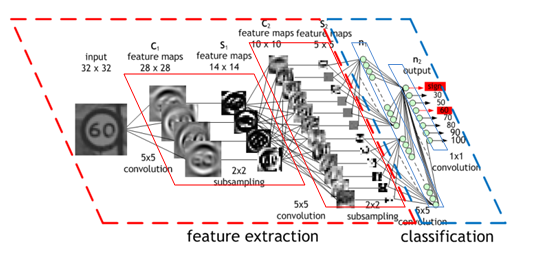
\includegraphics[scale=1.2]{dlarchitecture.png}
    \caption{Image by Maurice Peemen}
    \label{fig:dl-architecture}
\end{figure}

Moreover, it gave a strong impulse to the development of very efficient algorithms in the computer vision field. 
Indeed, nowadays there are a lot of tools that simplify the use of complex models trained to 
recognize hundreds of objects in an image. 

The so called fine-tuning technique allows net to recognize a different set of objects.
The purpose of fine-tuning is to reset the weights of final layers in a way that the model learned on some given features, can accomplish another task.
With this technique it will be just necessary to train final layers instead of the entire model for days and using large datasets.


\section{Pansharpening Applications}

Recently, a new pansharpening method based on a convolutional neural network has been proposed \cite{pnn}.
To accomplish that, it has been specialized a network built for super-resolution \cite{superesolution}.
From that model, other three different models have been tuned for GeoEye1, IKONOS and WorldView-2 sensors
with the aim of predicting the sensor characteristics and giving better performance. 

An important issue in this field is that it is difficult to found good images because of the high cost for high-resolution images.
For this reason, it cannot be possible to train deep network. The choice of the authors was to use three convolutional layers, illustrated in Fig.~\ref{fig:dl-pnn}.
The advantage of using only convolutional layers is that the input can have different sizes.

\begin{figure}[t]
    \centering
    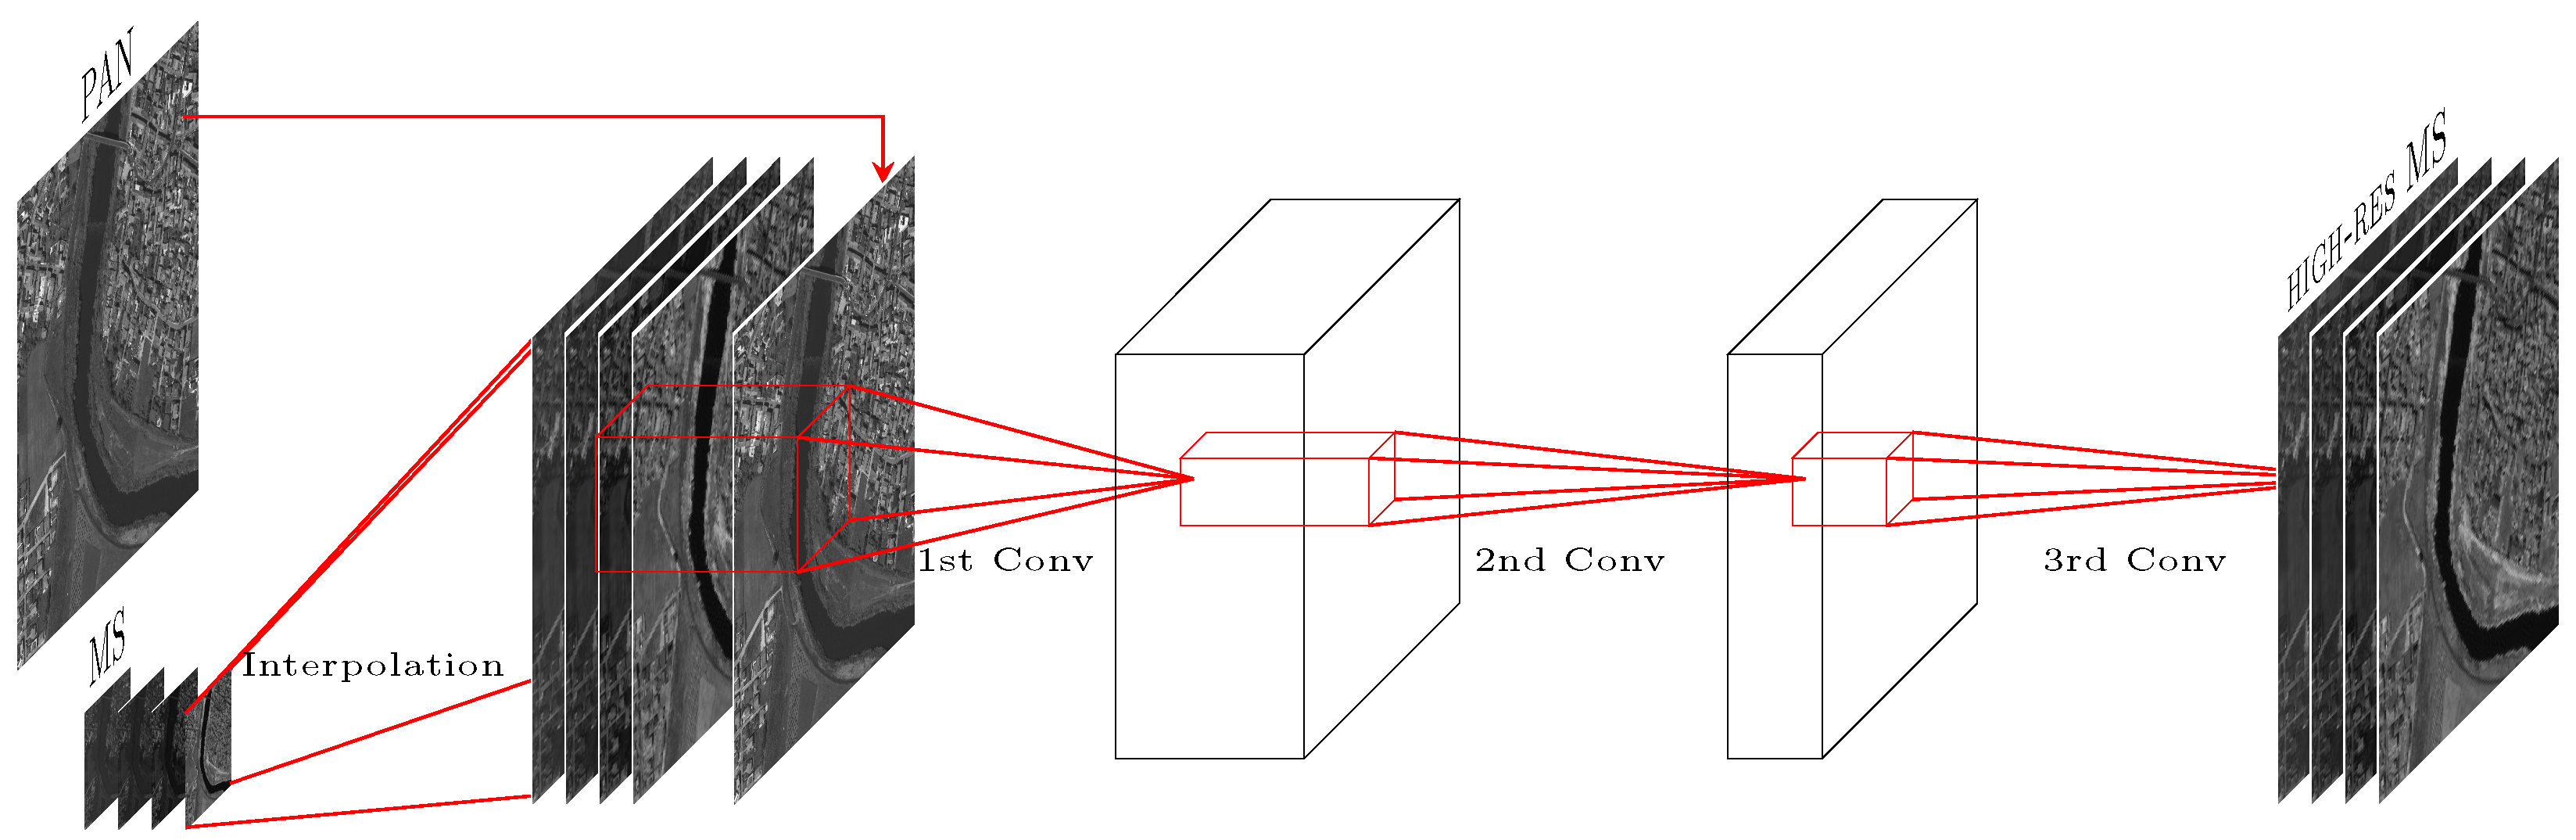
\includegraphics[scale=.8]{dl-pnn.png}
    \caption{CNN architecture for pansharpening\cite{pnn}}
    \label{fig:dl-pnn}
\end{figure}

The training phase showed in Fig.~\ref{fig:pnn-training} uses a reference approach in which the images are downsampled and fused. 
After the downgrande, the $P_L$ image is attached to the downgraded MS in order to provide input to the model.
The MSE error between the original MS and the network output are calculated and this error is used for the training of the weights.

\begin{figure}[t]
    \centering
    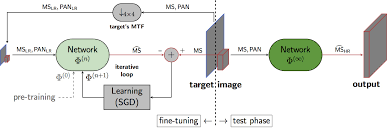
\includegraphics[scale=.9]{pnn-training.png}
    \caption{Training and Test\cite{pnn2}}
    \label{fig:pnn-training}
\end{figure}

Radiometric relevant indexes has been used to improve the results \cite{pnn}. 
It was showed that the network avoids learning the provided indexes.
Another important step introduced in \cite{pnn2} was to run a fast session of fine-tuning before the 
application of the model.
With the fine-tuning, the net can specialize the weights for the specific environment described by the downgraded image
and, subsequently, complete the fusion on the original images, with better results.
However, as described in the conclusions of \cite{pnn2}, performance with this approach is
not as much relevant as \textit{no-reference} approach that have a major impact to performance.
Another important disadvantage of the method is that when the model works with misaligned images, 
it is trained with images that have a fraction of the misalignment, depending on the scale ratio between PAN and MS. 

In another paper \cite{residualpnn}, the authors has tried different structures and strategies to improve the network released in \cite{pnn}.
An important result was achieved with a residual version of the original network.
The structure is showed in Fig. \ref{fig:residual-architecture}.

\begin{figure}[t]
    \centering
    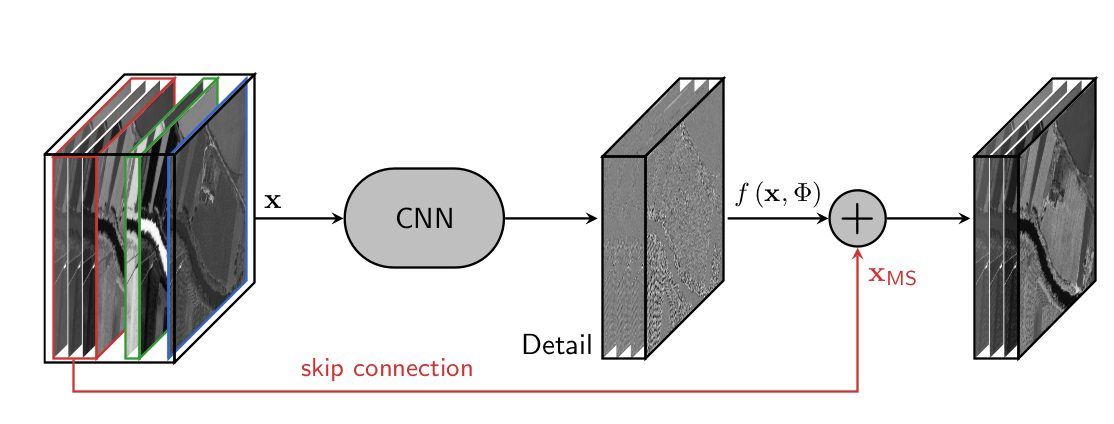
\includegraphics[scale=.35]{residualpnn-architecture.png}
    \caption{Residual-based version \cite{residualpnn}}
    \label{fig:residual-architecture}
\end{figure}

\begin{figure}[t]
    \centering
    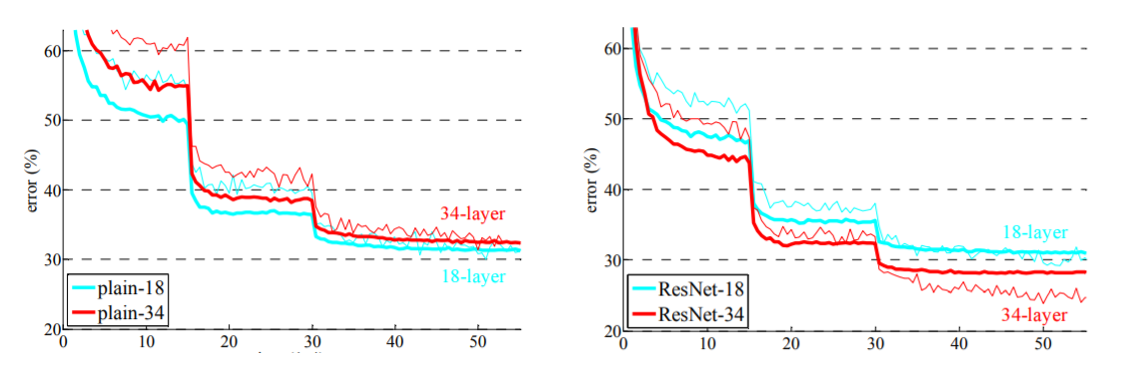
\includegraphics[scale=.35]{residual_comparison.png}
    \caption{Performance comparison between residual (right) and non residual (left) networks \cite{residual4}}
    \label{fig:residual-comparison}
\end{figure}

The residual version was not trained to reproduce the whole image,
but just the high-pass component. Indeed, the low-pass component is represented by the 
multispectral image provided by input. This means that the network reconstructs just the missing parts.

Residual-based structures were used in other papers \cite{residual1, residual2}, in particular in the DL in \cite{residual3, residual4}.

In conclusion, it was observed that it is easier to train a neural network for differences
instead of reproducing an ouput really similar to the input. 


The main results of \cite{residual4} are shown in Fig. \ref{fig:residual-comparison}.

\newpage

\chapter{Proposed Solution}

%\section{Introduction}

The aim of this chapter is to discuss and evaluate the difference between the training of the reduced resolution approach proposed in \cite{pnn}
and the training of the \textit{no-reference} approach developed in the research.
The analysis will cover the \textit{automatic differentiation} and the implementation in Tensorflow.

\section{Loss Function Issue}
\label{sec:lossfunction}
\begin{figure}[t]
    \centering
    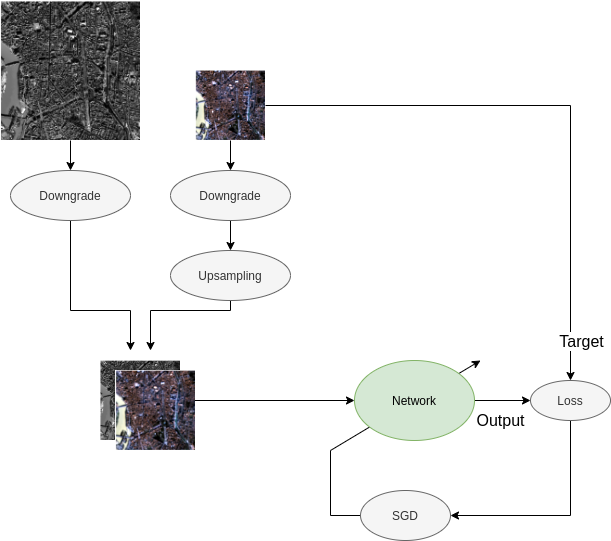
\includegraphics[scale=.45]{RRTraining.png}
    \caption{Graph of the training algorithm released by \cite{pnn}.}
    \label{fig:rrtraining}
\end{figure}

To assess the training set for the \textit{reduced resolution} (RR) method  described in \cite{pnn},
the algorithm synthesized in the Fig. \ref{fig:rrtraining} has been implemented.

Both PAN and MS are downsampled into two images called $MS_L$ and $PAN_L$.
The $MS_L$ is upsampled to match the $PAN_L$ size.
The images represent the input of the model that compute the error by the use of MS.
To update the model weights, a learning rate scheduler is used: the \textit{Stochastic Gradient Descent} (SGD)~\cite{sgd}.
A learning rate scheduler consent to modify the learning rate during the training
in order to optimize performance and reach easier the minimum error.
Other details about learning rate and learning rate scheduler can be find in the paragraph \ref{description}

\begin{figure}[t]
    \centering
    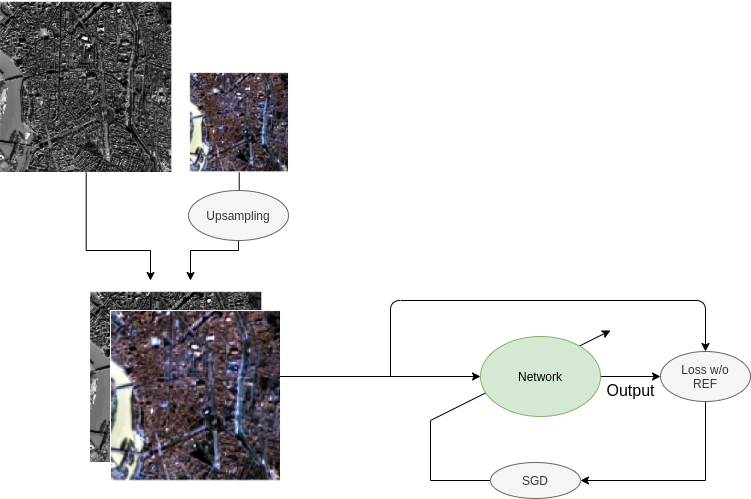
\includegraphics[scale=.45]{NOREFTraining.png}
    \caption{Graph of the training algorithm developed.}
    \label{fig:noreftraining}
\end{figure}

Instead of this procedure, we decided to use the \textit{no-reference} approach (NOREF) illustrated in Fig. \ref{fig:noreftraining}.
As the figure shows, the images are not downsampled. The great advantage is that 
the model is trained with original images and not with the downgraded version.
Also in this case, the MS is upsampled to match the PAN size.
Without the upsampling, it will not be possible to stack the images and apply the 3D filters of the convolutional layers.

In this case, the loss function does not use a target.
This is because the model is trained with the images at the highest possible resolution.
Indeed, the loss computation is done using a \textit{no-reference} index.
For this reason, this approach belongs into the \textit{unsupervised learning} field.
Oppositely to \textit{supervised learning}, unsupervised learning is a subfield of ML where the training process is not leaded by a target.





\section{Automatic Differentiation}
\textit{Automatic differentiation} is a set of techniques to efficiently calculate the gradient of a function by a computer.
Every computer program executes a sequence of elementary operations.
There are different kinds of techniques to differentiate a function: \textit{automatic differentiation}, \textit{numerical differentiation} and \textit{symbolic differentiation}.
The Fig. \ref{fig:differentiations} shows an example of all techniques that
evaluate the derivative of the same function. 
The various approach are described in the following.

\textit{Numerical differentiation} is the finite approximation of the derivatives.
\begin{equation}
    \frac{df(x)}{dx} \approx \frac{f(x+h) - f(x)}{h}
    \label{numdiff}
\end{equation}
%
In this technique, the computer evaluates the function described in Eq.~(\ref{numdiff})
at some sample points.
As described in \cite{autodiff}, this type of differentiation is easy to code.
However, the $O(n)$ cost of the evaluation in $n$ dimensions is so high
that ML, where $n$ can be millions or also billions, would not be accessible.

\textit{Symbolic differentiation} is a technique that uses the chain rule, the product rule and other rules to 
split the expression in known primitive derivative to obtain the result.
Eq.~(\ref{symbolicdiff}) shows how product rule and sum rule are applied:
%
\begin{equation}
    \begin{array}{l}
    \frac{d}{dx} (f(x) + g(x)) = \frac{d}{dx} f(x) + \frac{d}{dx}g(x) \\
    \frac{d}{dx} (f(x)g(x)) = \left(\frac{d}{dx} f(x)\right) g(x) + f(x)\left(\frac{d}{dx}g(x)\right)
    \end{array}
    \label{symbolicdiff}
\end{equation}
Techniques that belong to this class are really difficult to convert into a computer programs.

\textit{Automatic differentiation} systems explicitly split the operations in simplier ones and build a computation graph.
Each node of the graph have some attributes like values, primitive operations and parents.

Jacobian matrixes such as 
\begin{equation}
    J_f = \begin{bmatrix} 
        \frac{dy_1}{dx_1} & \dots & \frac{dy_1}{dx_n} \\
        \vdots & \ddots & \\
        \frac{dy_m}{dx_1} &        & \frac{dy_m}{dx_n}
        \end{bmatrix}
\end{equation}
are used to represent the derivative of each output $y$ respect to each input $x$ of a graph node.


%
For each primitive operation, it must be defined a \textit{Vector-Jacobian Product} (VJP). 
Combining all the VJP nodes, the result would be the value of the gradient.

\begin{figure}[t]
    \centering
    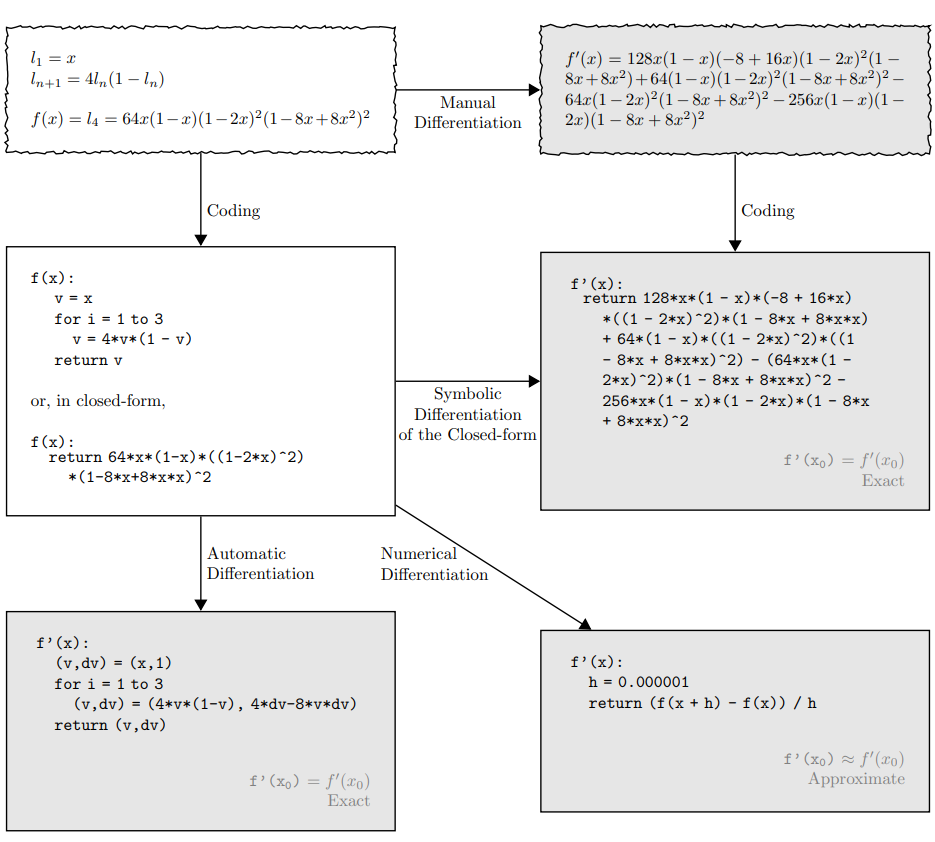
\includegraphics[scale=.4]{differentiations.png}
    \caption{Example with all type of differentiation \cite{autodiff}}
    \label{fig:differentiations}
\end{figure}

\textit{Automatic differentiation} provide different modes like \textit{forward mode} and \textit{reverse mode}.
In forward mode, \textit{automatic differentiation} and \textit{symbolic differentiation} are equivalent, as described in the paper \cite{auto_symbol}.
They both apply the chain rule and other differentiation rules and actually create expression graphs.
However, the first one was created specifically for the computer manipulation and includes numerical values. 
Indeed, the \textit{automatic differentiation} can handle also control flow statements like "if", "while" and "loops".
The second one, \textit{symbolic differentiation}, operates on mathematical expressions and symbols.

\section{Tensorflow and custom loss function implementation}
Tensorflow is the most famous ML and DL tool that implements the \textit{automatic differentiation}.
To build a custom loss function, Tensorflow provide APIs. These APIs define all the operations betweens \textit{Tensors} that are the basic datatype in Tensorflow.
The Tensorflow APIs used in the research code are showed in the Table \ref{tab:tensorflowapi}.
The external package \textit{tensorflow probability} APIs used are showed in Table \ref{tab:tensorflowprobability}.

After the definition of the custom loss function, at runtime Tensorflow translate the Python code in C/C++ for efficiency purpose, compile it, and builds the computation graphs.
Also, Tensorflow for a couple of years, integrate on it Keras, another framework that simplifie the creation of the model with 
all common layers well-defined into \texttt{Classes}.
To create a model it is necessary to create a \texttt{Model} class.
It is possible to add a layer using \texttt{model.add(Layer(args))}.
\texttt{Layer} is the corresponding class of the layer and args are the arguments like the input shape and the number of filters the layer should have. 
Firstly, using such a widespread framework has the advantage of a large community that supports challenging situations;
secondly, it will be a larger compatibility on Operating Systems, GPUs and hardware in general.


\begin{longtable}{ p{.30\textwidth} | p{.70\textwidth}} 
\caption{Table of tensorflow API used in the thesis.}\\
\hline
$abs(...);$ & Computes the absolute value of a tensor. \\

$add(...);$ & Returns x + y element-wise. \\ 

$cast(...):$ & Casts a tensor to a new type.\\

$constant(...):$ & Creates a constant tensor from a tensor-like object. \\

$divide(...);$ & Computes Python style division of x by y. \\ 

$expand_dims(...):$ & Returns a tensor with an additional dimension inserted at index axis. \\

$multiply(...);$ & Returns an element-wise x * y. \\ 

$ones(...):$ & Creates a tensor with all elements set to one. \\

$pad(...):$ & Pads a tensor. \\

$reduce\_mean(...);$ & Computes the mean of elements across dimensions of a tensor. \\ 

$reduce\_std(...);$ & Computes the standard deviation of elements across dimensions of a tensor. \\ 

$reduce\_sum(...);$ & Computes the sum of elements across dimensions of a tensor. \\ 

$sqrt(...);$ & Computes element-wise square root of the input tensor. \\ 

$square(...);$ & Computes square of x element-wise. \\ 

$squeeze(...):$ & Removes dimensions of size 1 from the shape of a tensor.\\
\hline
\label{tab:tensorflowapi}
\end{longtable}

\begin{longtable}{ p{.30\textwidth} | p{.70\textwidth}} 
\caption{Table of tensorflow probability API used in the thesis}\\
\hline
$stats.covariance(...);$ & Sample covariance between observations indexed by event\_axis. \\ 
\hline
\label{tab:tensorflowprobability}
\end{longtable}

\subsection{Loss Function}

At the beginning, to build the loss function, it was used a QNR approximation 

\begin{equation}
    f(x) = 1 - \widetilde{QNR}
    \label{loss}
\end{equation}
%
where $\widetilde{QNR}$ is the approximated QNR.

The $D_s$ and $D_\lambda$ were calculated using the Qavg, that is the average of Q indexes computed for each band. The Q index was calculated considering the whole image and not
dividing it into small patches.
The result shows a series of negative values instead of values between 0 and 1 as the original images format.
This is why the performance was unsatisfactory (results are illustrated in the Chapter \ref{chap4}).
Indeed, the model minimizes the loss functions (namely, it maximizes the QNR, considering \ref{loss}) no matter 
the sense of output values.
After some tests, it was considered to solve this problem using the $D_sreg$ described in \cite{dsreg} instead of $D_s$  
and migrate to an approximation of HQNR instead of the QNR.
Implementing the exact HQNR was unfeasible due to the difficulty on manupulating quaternions and hypercomplex numbers in TensorFlow in such
a way to keep the function differentiable.
In order to gain better performance, different versions of $D_\lambda$ indexes have been implemented, according to the diverse approaches proposed by the scientific community.

\chapter{Experimental results}\label{chap4}
\section{Description}
\label{description}
The implemented code has been written in Python 3.7 with the use of a file \texttt{main.py} as a entrypoint. 
It is compatible with Linux, Windows and MacOS and it can run on dedicated GPU as well as on CPU.

By the use of the standard \texttt{argparse} library, all the possible parameters can be codified on terminal.
This allows to run, with a bash file, all the experiments in series without changing the code.

At the beginning, the QNR function has been developed with approximations. 
In the Appendix \ref{qnr_functions}  the most important functions used for the QNR evaluation are presented.
As showed in the Appendix \ref{qnr_functions}, the Q index has been obtained as an average of the Q calculated band-by-band
instead of being calculated in patches as the original paper of the QNR described.
In order to obtain the spectral consistency measure $D_\lambda$, for each band of MS and fused image, 
it has been necessary the calculation of Q between bands, as formalized in Eq.~(\ref{ds}).
According to Eq.~(\ref{dl}), $D_s$ has been calculated as the Q between MS bands and $PAN_L$ and also between the fused image and the PAN.
This gives a quality measurements of the details inserted into the image. 

Due to the poor performance obtained via the QNR, it has been decided to use an approximation of HQNR. 
Approximations are due to the lack of Tensorflow hypercomplex API.
Instead of using Q4, for calculating $D_\lambda$, the Qavg used for the QNR has been adopted.
The $D_\lambda$ is thus calculated as 1 - Qavg, where Qavg is computed between the fused image filtered through a Gaussian filter and the MS.

Moreover, we employed as spatial distortion index the $D_sreg$ \cite{dsreg}, an implementation of the $D_s$ that takes advantages from the \textit{coefficient of determination} calculation. 
The coefficient of determination, also called \textit{R-squared} ($R^2$), is a statistical measure that represents the proportion of the variance for a dependent variable that is predictable from the indipendent variables.

The $D_sreg$ is obtained as $1 - R^2$, in which the coefficient of determination is calculated between the fused image and the PAN. 
The implementation is illustrated in the Appendix \ref{hqnr_functions}.
Depending on the sensor used for the image acquisition, the filter would be different to match the sensor MTF.
The filters were created with the Matlab Toolbox, exported in the \texttt{.mat} format and imported in the project at runtime.
It was decided to use no padding after the filtering process and cut the pixels affected by border effects from the MS during the Q calculation.  

An important choice regarded the learning rate. The learning rate is multiplied with the gradient of the error for each layer
and it will determines how quickly the error decrease. 

If the learning rate is too high, the error will drop down quickly, but difficulties will be encountered in finding minimum.
With a too low learning rate, it can take long time to reach the convergence or the algorithm gets stuck in a local minimum.
According to the community, the best approach is to use a learning rate scheduler like Adam \cite{adam} or SGD \cite{sgd}.
At the start of the training, the model can have a high learning rate so that it can explore all the loss function.
After that, the learning rate will be gradually decreased to avoid oscillations.
The learning rate is one of the parameters that requires some experiments to be tuned.
The best case is to reach the maximum possible quality with a constant increase in performance during the training.
The main index of performance was Q2N. At the moment, Q2N is the best index used with reference image.
It is important in the training to avoid a bell shape in the index graph. Bell shape indicates that the Q2N increases really fast at the beginning.
After reaching the pick value of optimum, it decreases really fast. 
This characteristic would made the training difficult in real applications.
The reason why is that the calculation would be impossible due to the unavailability of the reference image.

Without the bell shape during the training, the model can only have an increase in performance.


\section{Experimental Settings}

\begin{figure}[t]
    \centering
    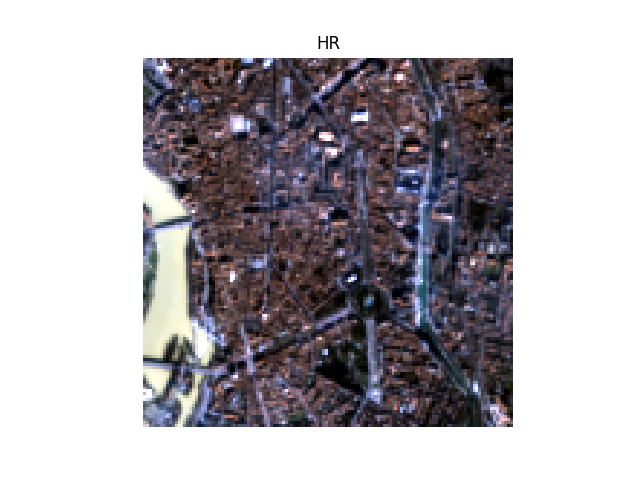
\includegraphics[scale=.5]{toulouse.png}
    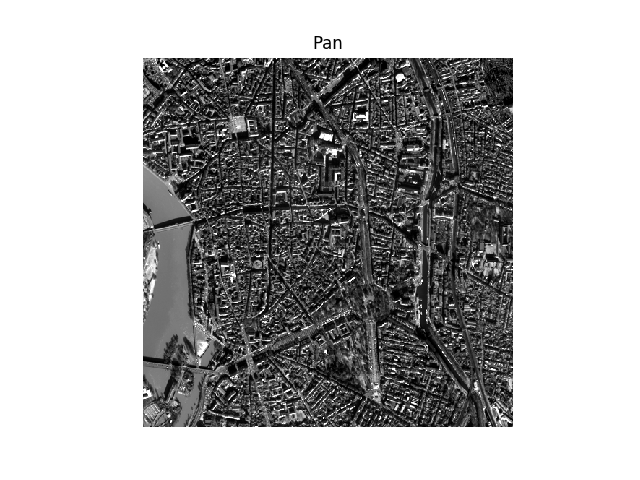
\includegraphics[scale=.5]{toulouse_pan.png}
    \caption{Multispectral and Panchromatic Toulouse images used for all the tests}
    \label{fig:toulouse}
\end{figure}


All types of training have been executed in a test image illustrated with a true color representation in Fig. \ref{fig:toulouse} and identified as Toulouse dataset.
The Toulouse dataset is a couple of IKONOS images acquired over the city of Toulouse, France, in 2000.
The MS sensor acquires an image of 512$\times$512 pixels in the visible and near-infrared spectrum range in 4
different bands and with a 4m spatial sampling interval (SSI). 
The pancromatic image is constituted by an image of 2048$\times$2048 pixels with a 1m SSI.

DL models should not be specialized too much for the training set otherwise, the model could have low performance for new data not included in the training set.
To avoid this situation, it is necessary to create a validation set in which there are different data. 
Performance on the validation set are more similar to real world performance.
The validation process is described in the Fig. \ref{fig:validation}.

\begin{figure}[t]
    \centering
    \includegraphics[scale=.5]{validation.png}
    \caption{Validation process}
    \label{fig:validation}
\end{figure}

To generate a reference image for the quality assessment, MS and PAN has been downsampled.
The original MS has been used as Ground Truth (GT).

At every epoch, the downsampled images $PAN_L$ and $MS_L$ were used 
to produce a fused image with the updated weights and compared with the GT.
This means that the images will constitute the validation set. 
Reference indexes like SAM, ERGAS and Q together with \textit{no-reference} indexes QNR and HQNR were calculated between the output of the model and the GT.
Those indexes has been obtained with the MatLab toolbox functions provided by \cite{criticalComparison} and MatLab engine 
for Python \cite{matlab}.
The procedure can give a real performance assessment of the whole model.
The training set have always better performance as the model optimizes the 
error of these data. It needs to be highlighted that only the performance of the validation set are relevant. 

For the training in RR approach, as described in the Paragraph \ref{sec:lossfunction}, the $PAN_L$ and $MS_L$ are downsampled again as the model
would have a different target from GT.
Training the model with the GT as target have no valid applications.
In real world, the model would not have a GT.
Additionally, the validation set would have no relevant performance as the model is trained with the same data.

It has been noticed that, for some images, the model that uses the fine-tuning with the reference approach has worse performance than the original one.
The reason is that the model is fine-tuned with the downgraded images.

The characteristics of the sensors, in general, do not satisfy the scale invariance hypothesis and downsampling the input does not guarantee similar performance like using the original images
as described also in the previous chapters.

In the NOREF approach, the images are not downsampled again as the model use a \textit{no-reference} loss function.

To compare the different methods, the model has been also trained with the GT image itself using the MSE loss function.
The purpose is to compare the previous described methods with the best possible solution; however it is not applicable in a real approach.

\section{Results}
\begin{figure}[t]
    \centering
    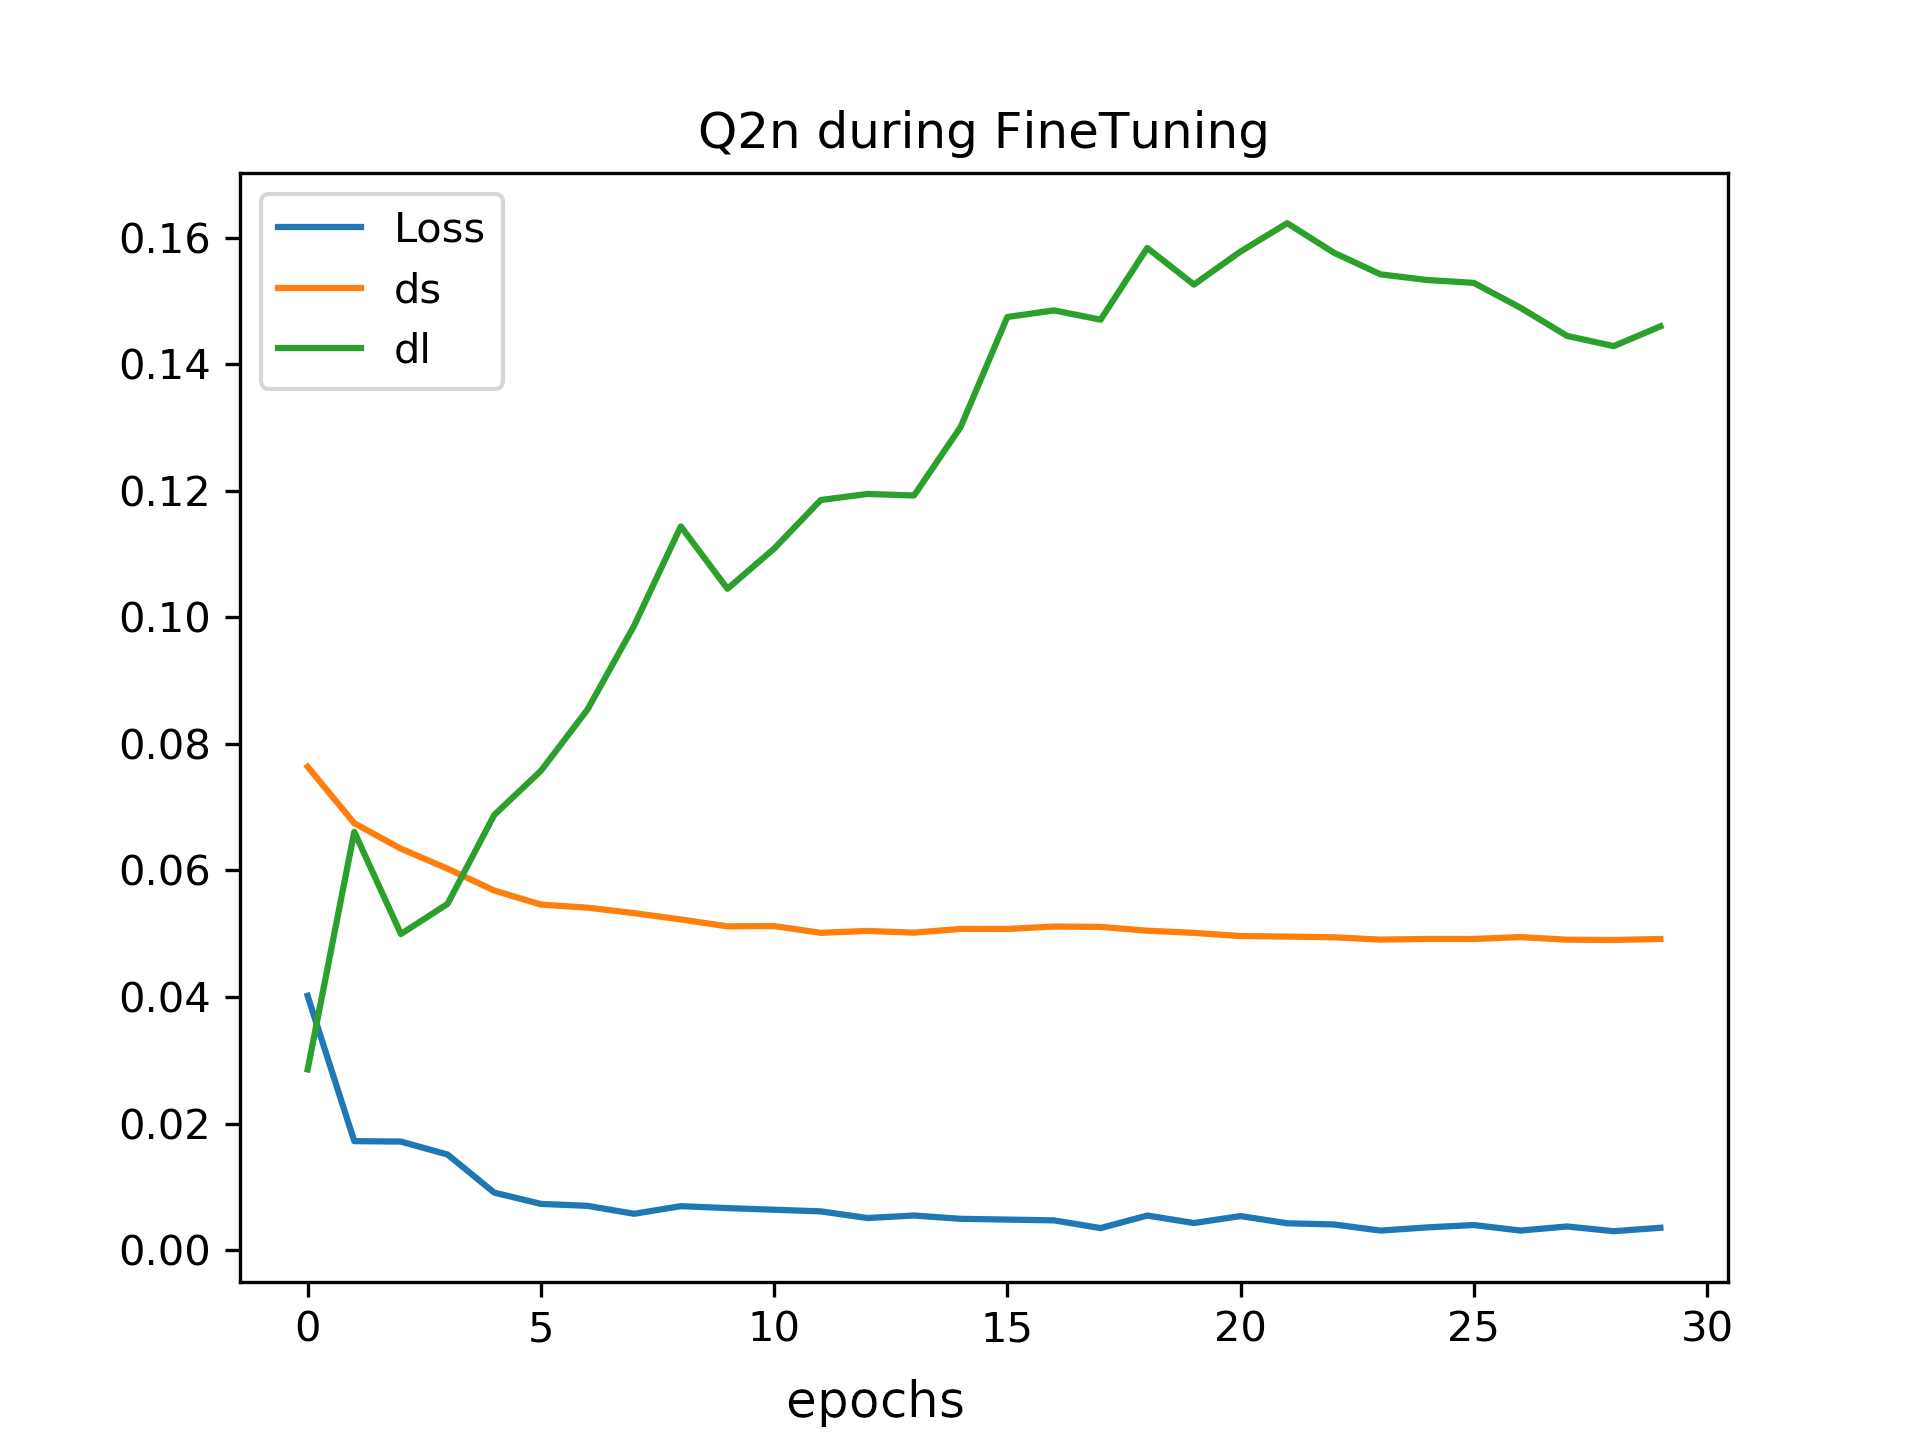
\includegraphics[scale=.7]{qnr1.png}
    \caption{Values of Loss, DS and DL of QNR during the training.}
    \label{fig:qnr1}
\end{figure}


\begin{figure}
    \centering
    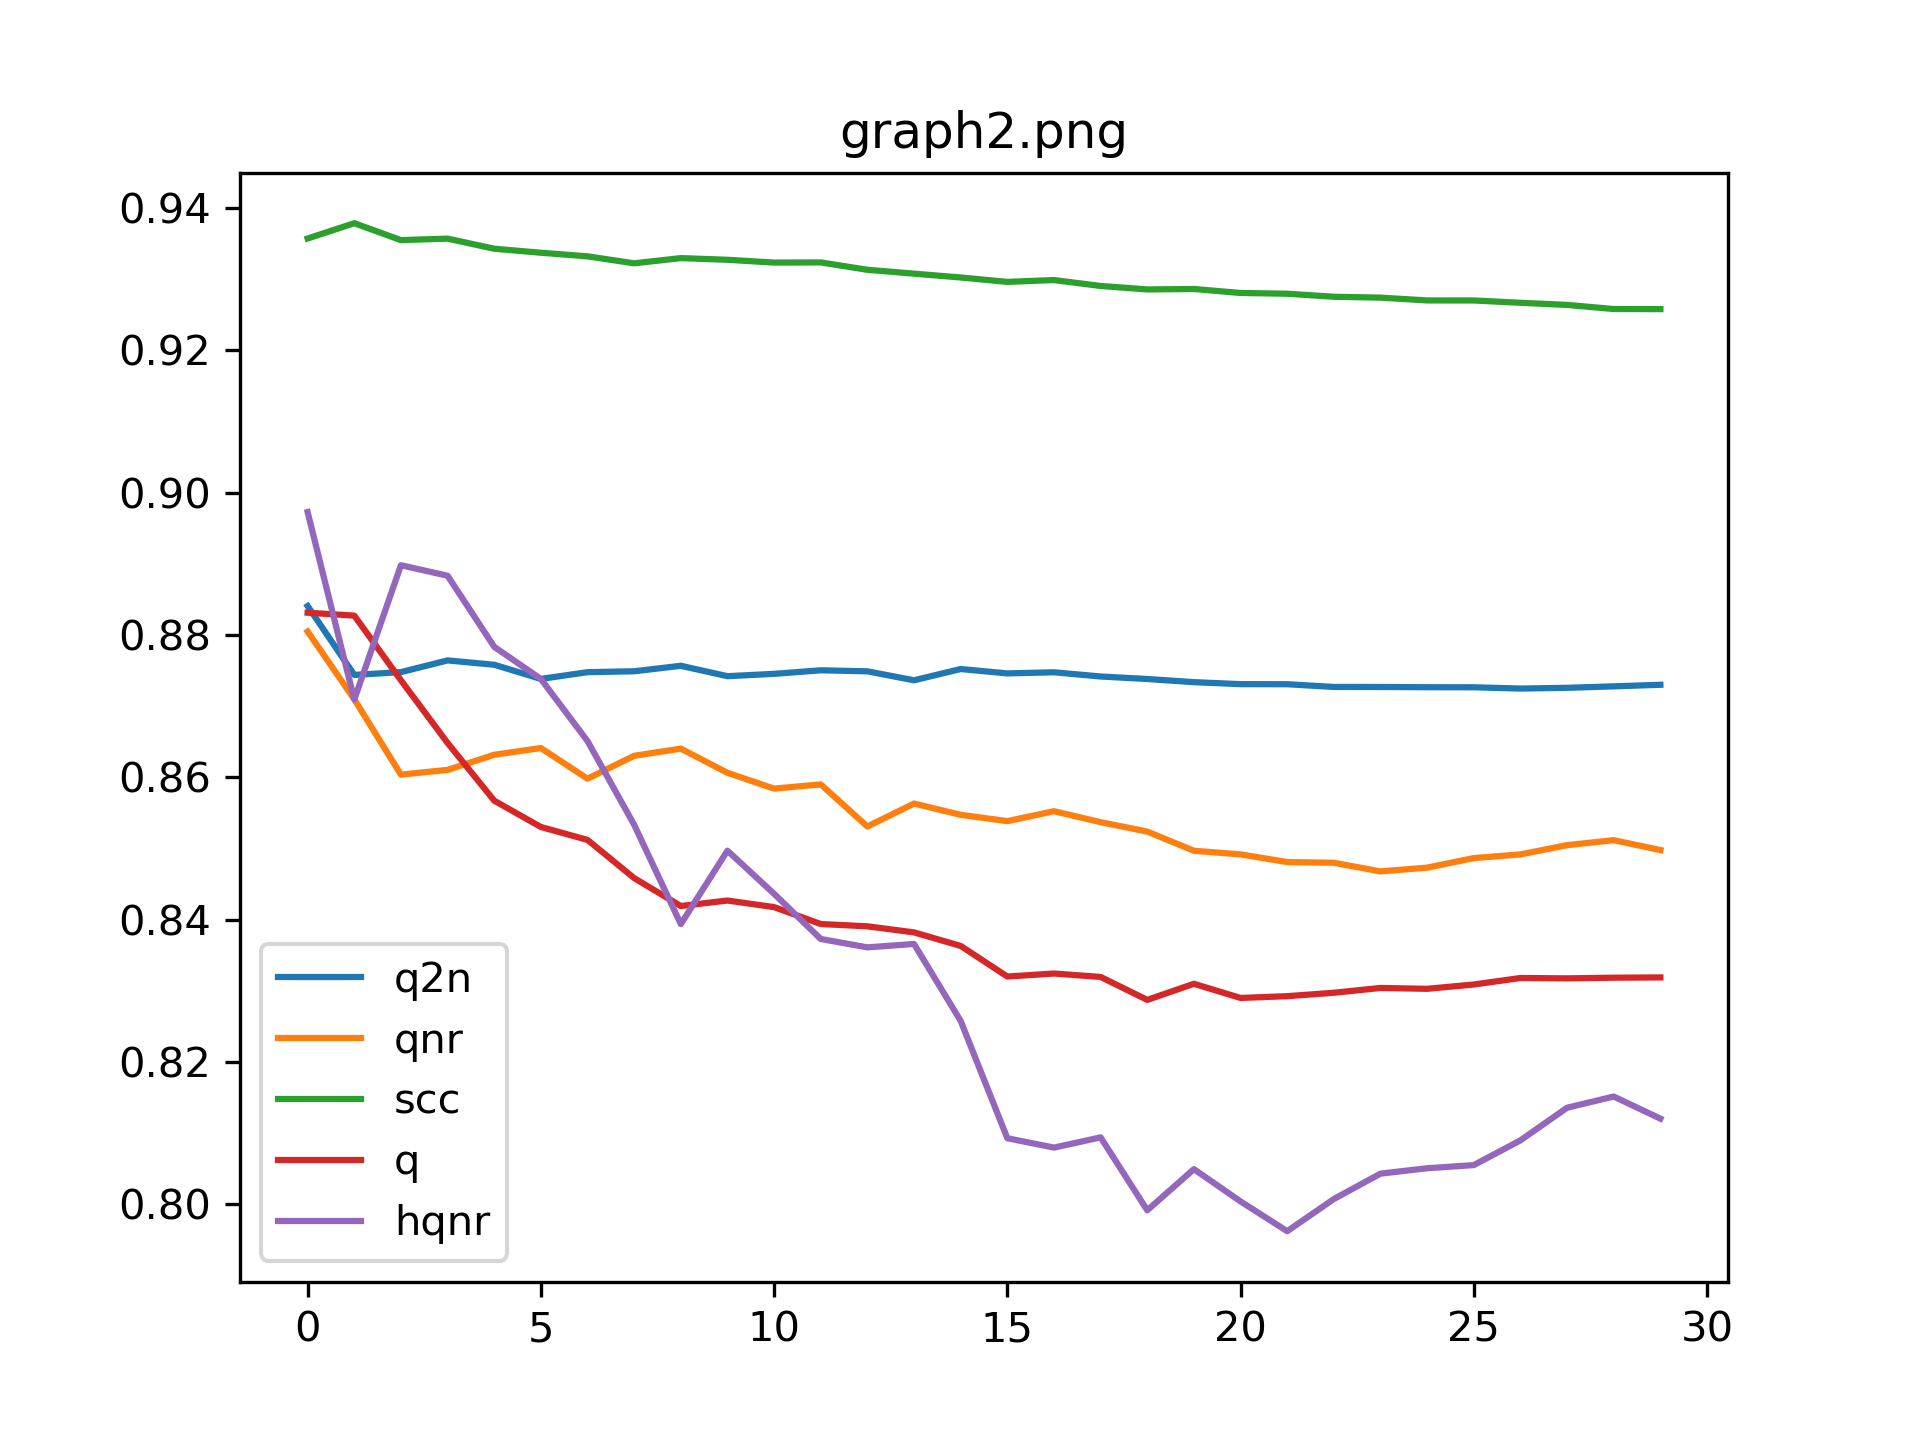
\includegraphics[scale=.7]{qnr2.png}
    \caption{Values of Q2N, QNR, SCC, Q and HQNR during the training.}
    \label{fig:qnr2}
\end{figure}


\begin{figure}
    \centering
    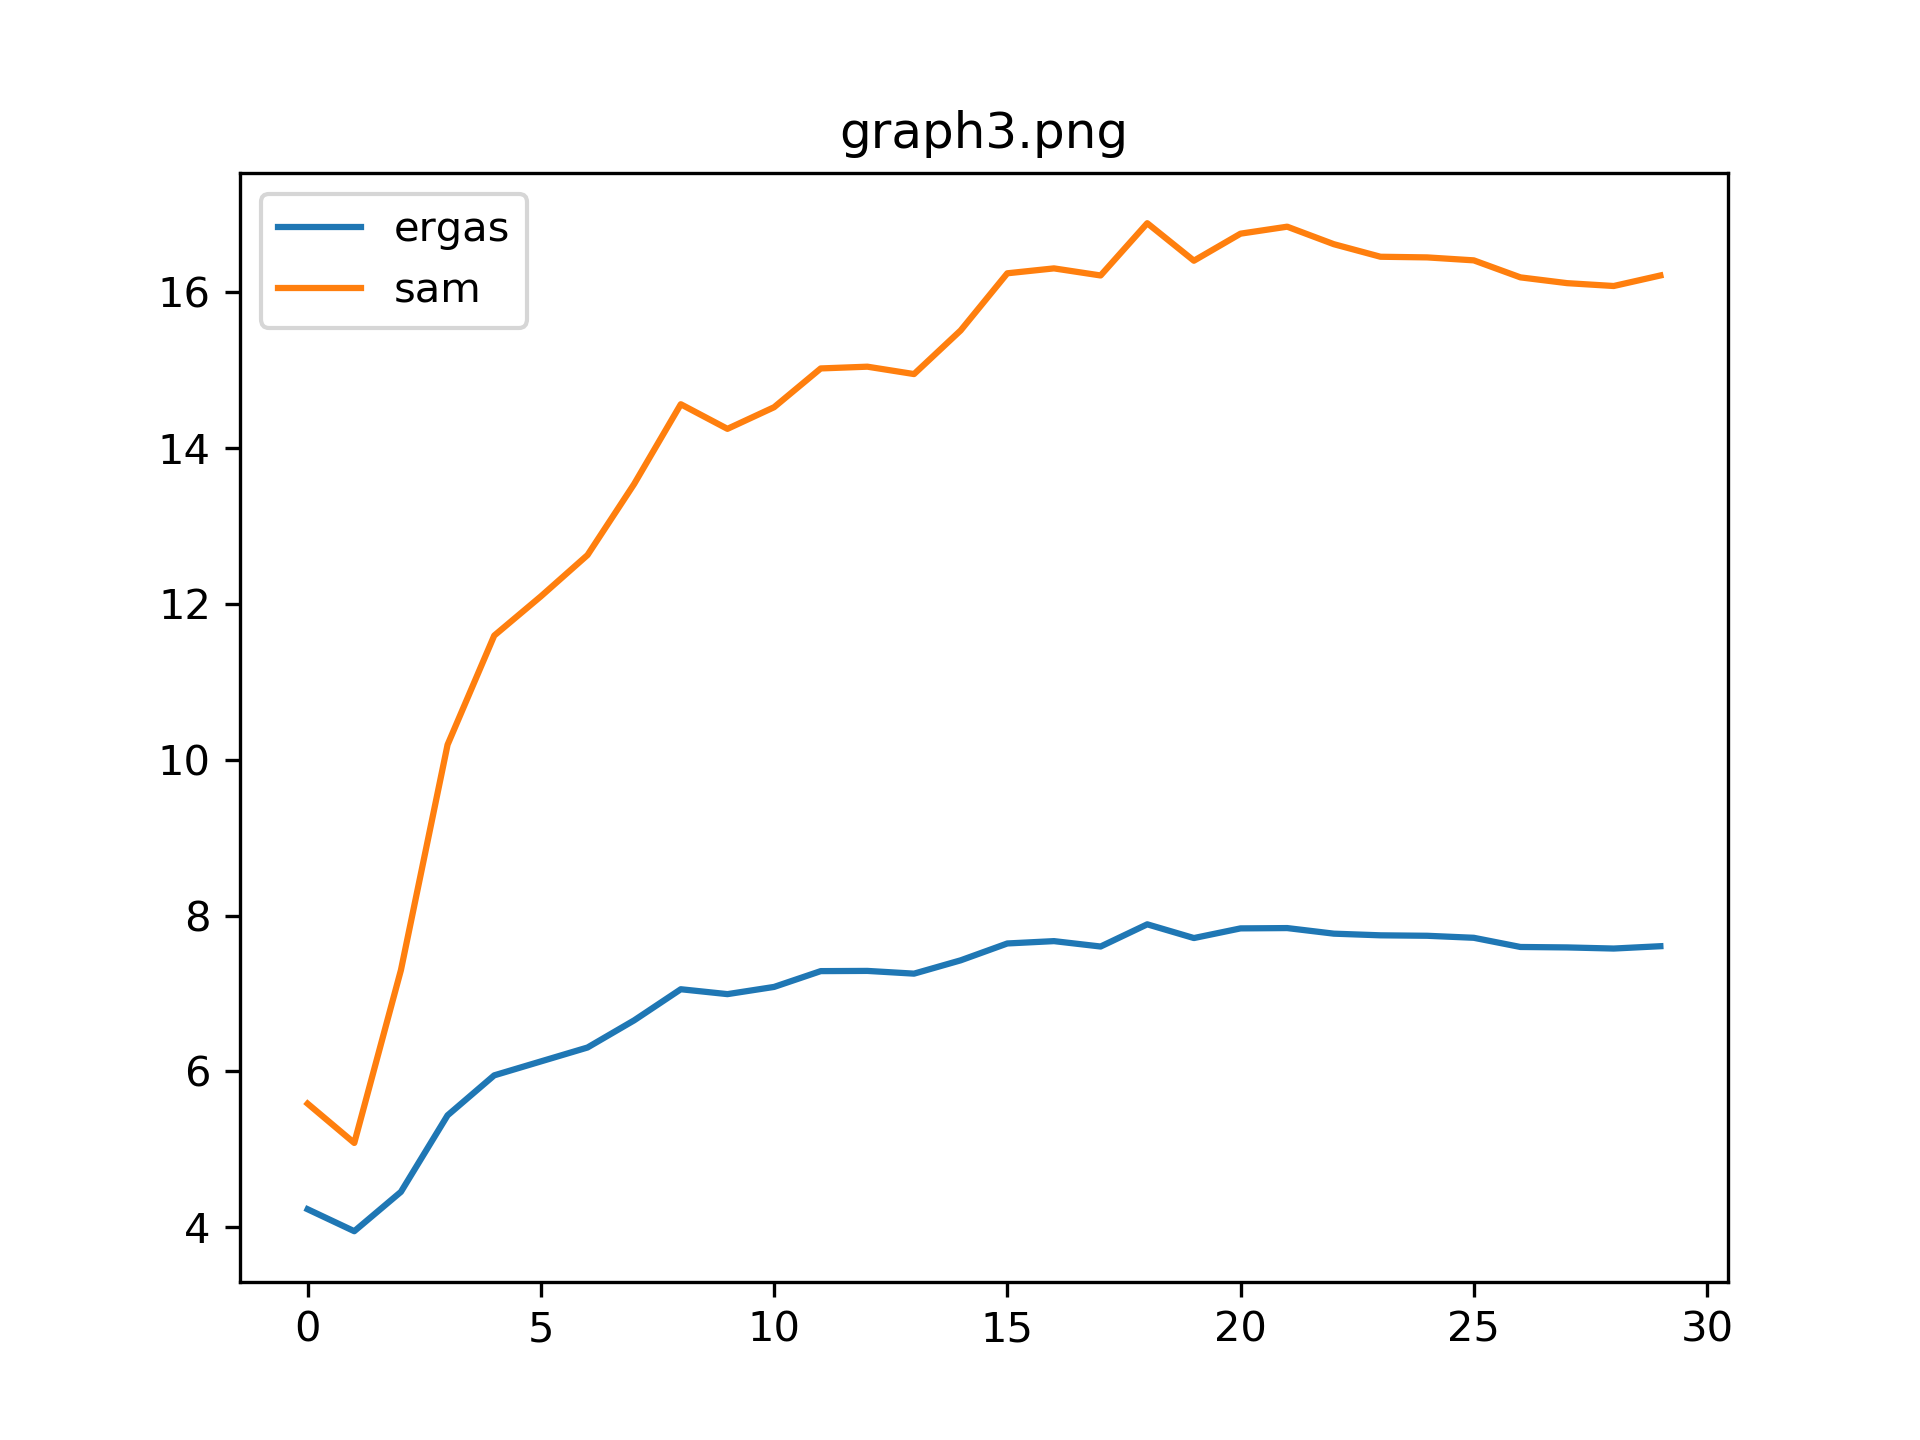
\includegraphics[scale=.7]{qnr3.png}
    \caption{Values of ERGAS and SAM during the training.}
    \label{fig:qnr3}
\end{figure}

The use of the classical QNR function, whose formula is given by Eq.~(\ref{qnr})), has produced no appreciable results.
During the training, while the error continues to decrease, the image quality indexes computed through the Matlab Toolbox get worse, as showed in Fig.~\ref{fig:qnr1},~\ref{fig:qnr2} and~\ref{fig:qnr3}, even the QNR itself.
The reason is related to the fact that, in order to minimize the error, it has been generated an image with negative values.
An input with negative values is not expected by any of the indexes used.
This creates a discrepancy between the QNR used in the loss function and the QNR of the Matlab Toolbox.
Indeed, with inputs having values between 0 and 1, the QNR developed in Tensorflow and the Matlab one returns the same results.
In other words, the loss tends to reach his minimum value even though this is not reflected in an increase of the quality indexes. 

\begin{figure}[t]
    \centering
    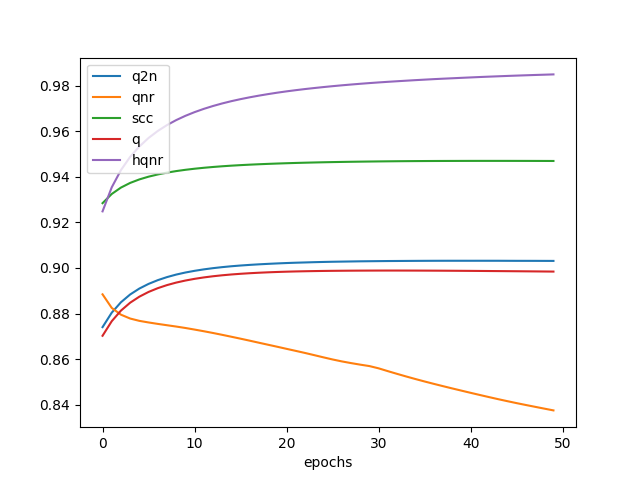
\includegraphics[scale=.7]{toulouse_noref.png}
    \caption{Values of Q2N, QNR, SCC, Q and HQNR during the training using the loss function with HQNR.}
    \label{fig:hqnr1}
\end{figure}

\begin{figure}[t]
    \centering
    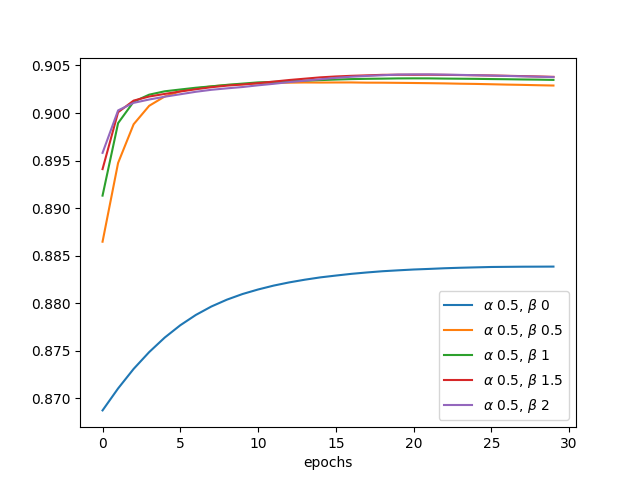
\includegraphics[scale=.7]{alpha_beta1.png}
    \caption{Learning curves obtained by varying $\beta$ with a 0.5 step in the range $[0,2]$ and $\alpha$ set to 0.5.}
    \label{fig:alpha_beta1}
\end{figure}

After those tests, it has been decided to change the loss function using another \textit{no-reference} index, the HQNR, whose expression is reported in Eq.~(\ref{hqnr}).
However, this index is more complex than the QNR, as it involves quaternions and operations with hypercomplex numbers.

For this reason, it was applied an approximated version of HQNR that is fully described in the previous chapter. The results obtained for the Ikonos Toulouse dataset are shown in Fig.~\ref{fig:hqnr1}. 

With this type of loss function, it was recorded a performance improvement in terms of all the indexes, except the QNR.
The latter, as evidenced also by the previous results, does not seems to be a good index for the quality assessment.

To explore the behavior of the training algorithm for different values of the coefficients $\alpha$ and $\beta$ that are present in Eq.~(\ref{hqnr}), several tests have been carried out by firstly modifying the parameters with steps of 0.5. 
An interesting trend has been noticed with $\alpha$ equal to 0.5 and results of those tests are available in Fig.~\ref{fig:alpha_beta1}.
Furthermore, tests with $\alpha$ set to 0.5 and $\beta$ ranging from 0.5 to 2 with 0.25 steps have been carried out. The results are showed in Figs.~\ref{fig:alpha_beta3} and~\ref{fig:alpha_beta4}. The close-up provided from the latter figure allows to conclude that the best results are obtained with $\alpha=0.5$ and $\beta=1.75$. 



\begin{figure}
    \centering
    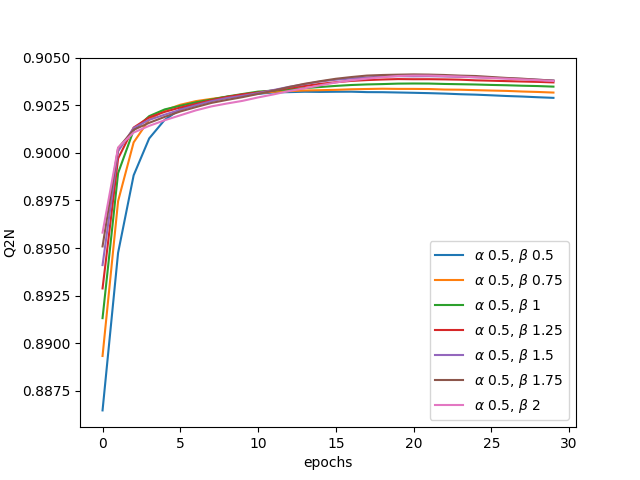
\includegraphics[scale=.7]{alpha_beta3.png}
    \caption{Learning curves obtained by varying $\beta$ with a 0.25 step in the range $[0.5,2]$ and $\alpha$ set to 0.5.}
    \label{fig:alpha_beta3}
\end{figure}

\begin{figure}
    \centering
    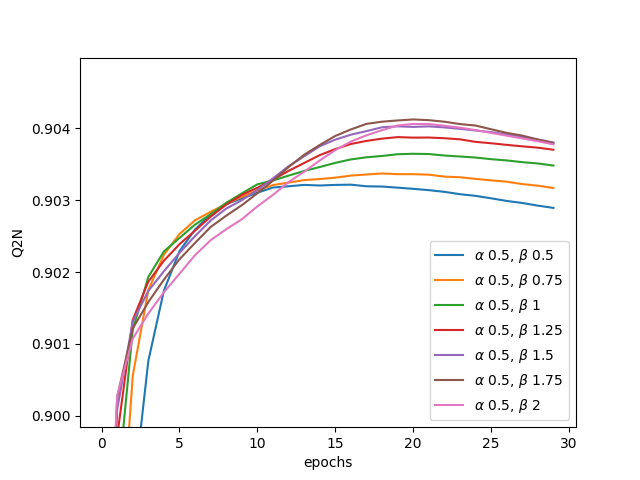
\includegraphics[scale=.7]{alpha_beta4.png}
    \caption{Zoom of Fig. \ref{fig:alpha_beta3} with Q2N in the range [0.9, 0.905].}
    \label{fig:alpha_beta4}
\end{figure}

\begin{figure}[t]
    \centering
    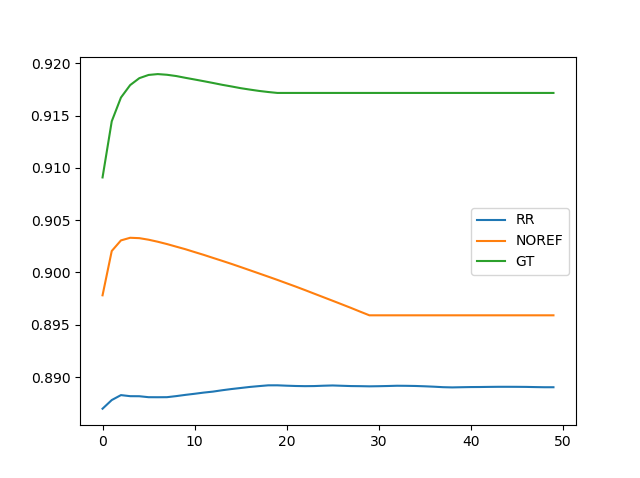
\includegraphics[scale=.7]{toulouse_gt_rr_noref.png}
    \caption{Q2N experiment results with GT, RR and NOREF.}
    \label{fig:gt_rr_noref}
\end{figure}

After these experiments aimed at selecting the optimal values for the proposed approach, a comparison with existing techniques has been carried out.
In particular, the GT method uses the \textit{ground truth} during the training and is thus introduced as a reference since it cannot be employed in the practice;
instead, RR denotes the method used in \cite{pnn} with reduced resolution training. 
The method proposed in this work that uses full-resolution images and is described in the previous paragraphs is here denoted as NOREF.


Fig. \ref{fig:gt_rr_noref} shows the comparison between the three different methodologies. 
The graph indicates that the Q2N trend (in green) of the GT approach has a high margin of performance over the others. The expectation was that the model would reach a level close to 1. However, with the actual architecture, the model cannot achieve higher performance.
Worst performance has been obtained by RR (in blue) where the trend increases in the first two epochs and then remains stuck below 0.89. 
The NOREF method (in yellow) yields a continuous growth and remains constant from the 30th epoch onwards. 
The model has better performance than RR despite his recent application.



\begin{figure}
    \centering
    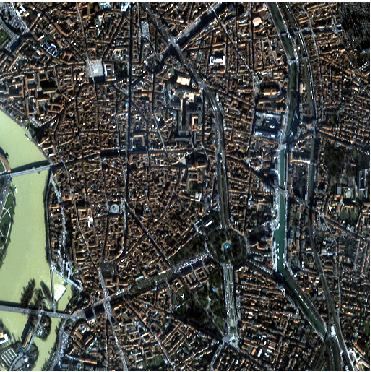
\includegraphics[scale=.8]{Target.png}
    \caption{Ground Truth used for validation}
    \label{fig:comparison_target}
\end{figure}

\begin{figure}
    \centering
    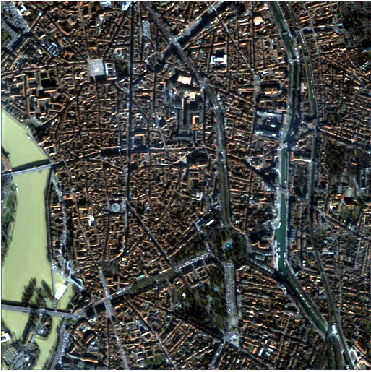
\includegraphics[scale=.8]{GT.png}
    \caption{Result of GT method}
    \label{fig:comparison_gt}
\end{figure}

\begin{figure}
    \centering
    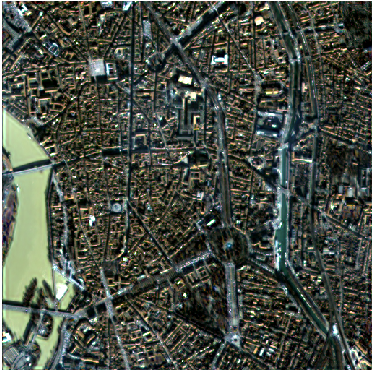
\includegraphics[scale=.8]{NOREF.png}
    \caption{Result of NOREF method}
    \label{fig:comparison_noref}
\end{figure}

\begin{figure}
    \centering
    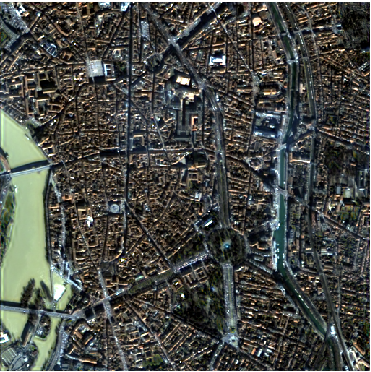
\includegraphics[scale=.8]{RR.png}
    \caption{Result of RR method}
    \label{fig:comparison_rr}
\end{figure}

\bb{In Figs. \ref{fig:comparison_gt}, \ref{fig:comparison_noref}, \ref{fig:comparison_rr} the images obtained with GT, NOREF and RR methods are illustrated respectively.
The images show some border effects noticeable primarily on the left border. Those effects are introduced since the prediction of the model (high pass component) that have a reduced size is added to the MS image used for the image (low pass component). 
The convolutional layers of the network reduce the size of the output layer-by-layer depending on the used kernel. In particular, the model used for the experiments decreases the image by 6 pixels per side.}

\begin{figure}
    \centering
    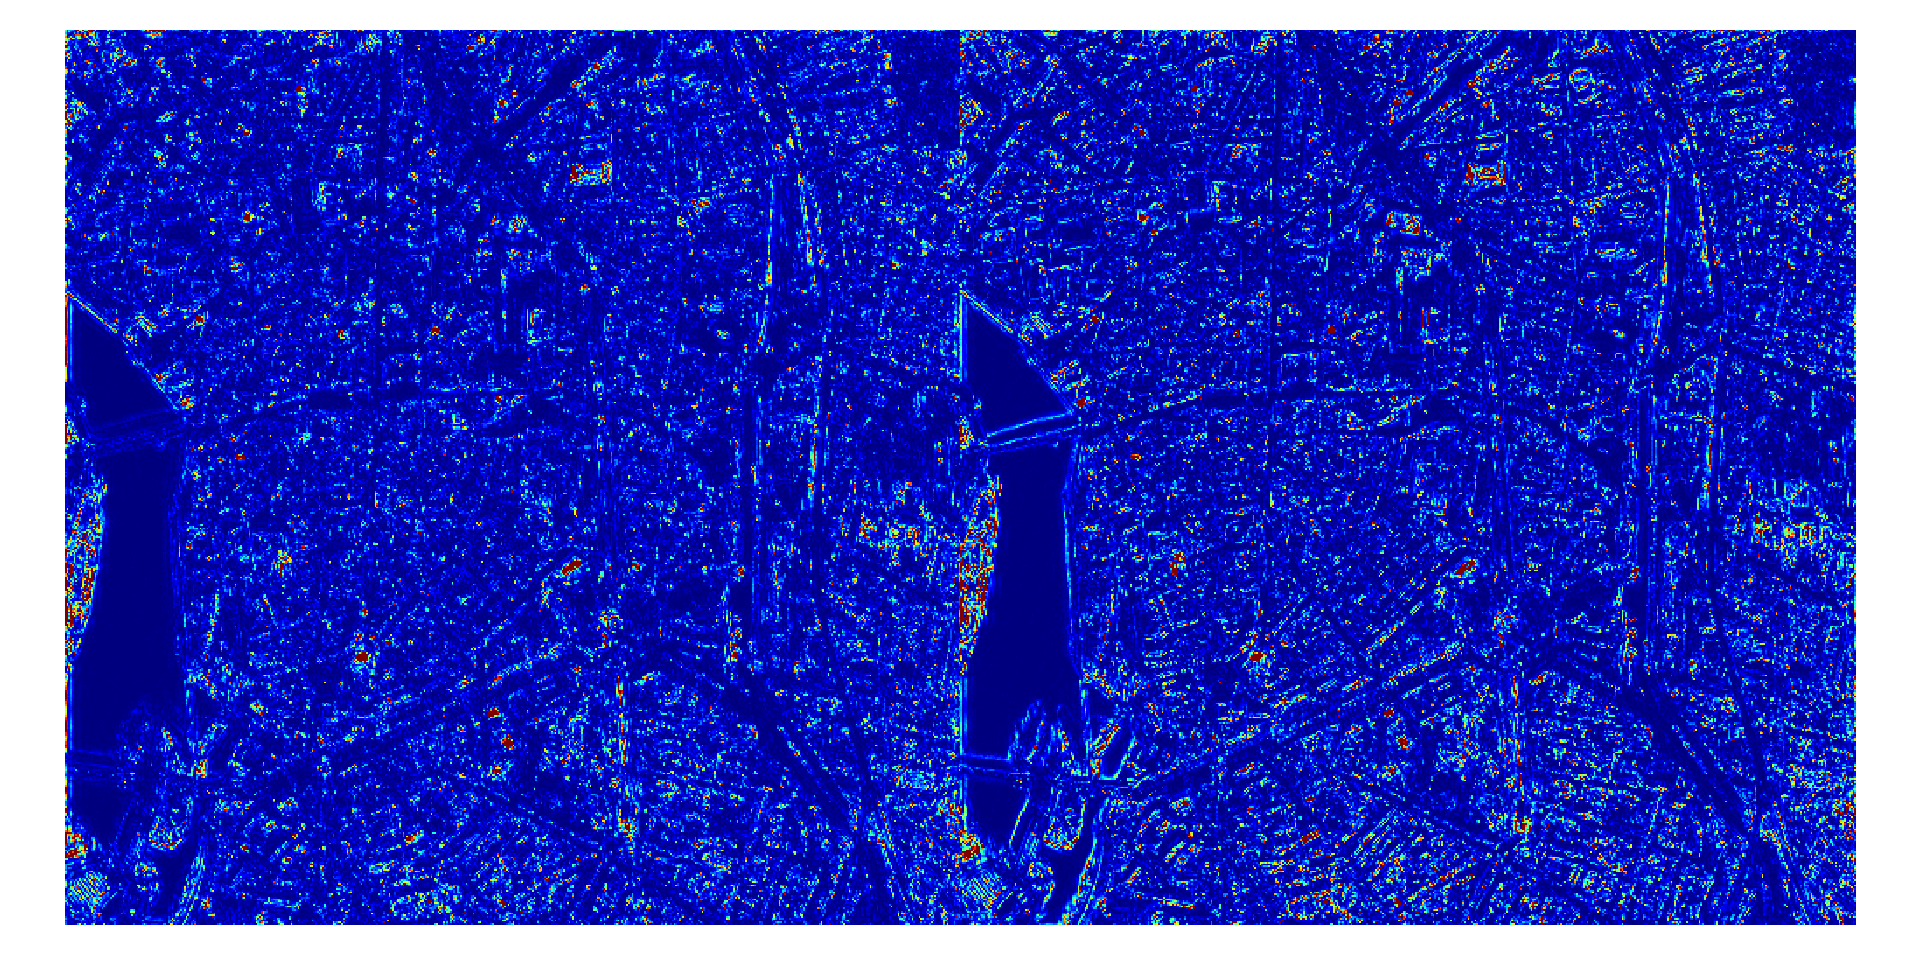
\includegraphics[scale=.35]{diff_PAN_NOREF_RR.png}
    \caption{Images representing the channels sum of the difference between NOREF and RR with ground truth}
    \label{fig:diffcolors}
\end{figure}

\bb{For a better visual inspection, the differences of NOREF and RR with the ground truth are showed in the Fig. \ref{fig:diffcolors}
The figure emphasise with red and yellow the significant errors and with blue the areas the negligible ones.
The RR difference image shows some red spots on the bottom and on the center but in the NOREF these areas are processed in a better way}


\chapter*{Conclusions}
\addcontentsline{toc}{chapter}{Conclusions}
In this work, we started from the recently proposed \cite{pnn2} CNN-based pansharpening method and, using modern and more compatible tools, explored a \textit{no-reference} approach.
This opened numerous issue regarding the loss function to choose.
Without a target for the model, the loss function became the critical aspect more than before.

In the current study, we implemented new training and validation processes that do not make use of a reference image (NOREF) and compared them with existing and reference approaches. 
It was demonstrated that the use of the QNR index as full resolution loss is not appropriate, since it does not provide valuable results in this settings. On the contrary, we developed an approximate implementation of the HQNR index that obtains better performance than the widespread training operating at reduced resolution (RR). It was also shown, by resorting to an ideal training scheme based on the ground truth (GT), that there is room for further improvements. 

It is arguable that the use of a hybrid RR and NOREF approach can have even better performance as it inherits the best aspects of both methods.
Indeed, a hybrid model would use reduced resolution images with a robust reference index
and, at the same time, images at the original resolution would compensate any problems due to the different behavior of the algorithms across scales.

Furthermore, different architectures can be considered.
In fact, an architecture with only convolutional layers includes a limited number of filters and every filter is applied to the whole image.
This implicates that a single filter is trained at each level by optimize the performance on the whole image instead on a particular area.
Images can have different environments (like rural or urban) and the model could benefit by neurons divided to specialize different patches.

This results can be achieved with different techniques.
At first glance, it would be possible to generate multiple small models, which are fine-tuned for patches.
Furthermore, changing the model layers would deliver images processed in a specialized way.
To this extent, in a dense layer, all neurons have their own specific weights that would be trained for the exact pixels in input.
Indeed, the actual limit in \textit{pansharpening neural networks} (PNN) is treating images without considering the different morphology of them.

For these reasons, the current research lay the foundation for future development in the field of pansharpening.
A \textit{no-reference} model with a more implemented and specialized image processing can overcome the limits of the model in use.
\newpage

\bibliographystyle{unsrt}
\bibliography{references}

\newpage


\newgeometry{margin=1in}

\appendix

\begin{spacing}{1}
    \chapter{Python implementation of no-reference quality indexes }
        \section{QNR}
        \label{qnr_functions}
        \lstinputlisting[language=python]{qnr.py}

        \section{HQNR}
        \label{hqnr_functions}
        \lstinputlisting[language=python]{hqnr.py}
\end{spacing}

\restoregeometry

\end{document}

